\documentclass[11pt,a4paper]{article}
\usepackage{fontspec}
\setmainfont{texgyretermes}[Extension=.otf,UprightFont=*-regular,BoldFont=*-bold,ItalicFont=*-italic,BoldItalicFont=*-bolditalic]
\setsansfont{texgyreheros}[Extension=.otf,UprightFont=*-regular,BoldFont=*-bold,ItalicFont=*-italic,BoldItalicFont=*-bolditalic]
\setmonofont{lmmono10}[Extension=.otf,UprightFont=*-regular]
\usepackage[a4paper,margin=2.2cm]{geometry}
\usepackage{graphicx,booktabs,tabularx,array,amsmath,amssymb,float,enumitem,xcolor}
\usepackage[font=small,labelfont=bf]{caption}
\usepackage[most]{tcolorbox}
\usepackage[colorlinks=true,linkcolor=teal!60!black,urlcolor=teal!60!black,citecolor=teal!60!black]{hyperref}
\usepackage{titlesec}
\usepackage{tikz}
\usetikzlibrary{positioning,arrows.meta,calc}

\definecolor{acc}{HTML}{2A78D6}
\definecolor{org}{HTML}{EB6834}
\titleformat{\section}{\Large\sffamily\bfseries\color{acc!75!black}}{\thesection}{0.6em}{}
\titleformat{\subsection}{\large\sffamily\bfseries}{\thesubsection}{0.5em}{}
\titlespacing*{\section}{0pt}{12pt}{5pt}
\titlespacing*{\subsection}{0pt}{8pt}{3pt}
\setlist{itemsep=2pt,topsep=3pt}
\renewcommand{\arraystretch}{1.18}
\newtcolorbox{ghichu}[1][Điểm cần nhớ]{colback=acc!5,colframe=acc!70!black,fonttitle=\sffamily\bfseries,title=#1,
  boxrule=0.6pt,arc=2pt,left=6pt,right=6pt,top=4pt,bottom=4pt}
\captionsetup{justification=raggedright,singlelinecheck=false}
\graphicspath{{figs/}}
\renewcommand{\figurename}{Hình}
\renewcommand{\tablename}{Bảng}
\renewcommand{\refname}{Tài liệu tham khảo}
\renewcommand{\abstractname}{Tóm tắt}
\setcounter{topnumber}{3}\setcounter{totalnumber}{4}\renewcommand{\topfraction}{0.9}\renewcommand{\textfraction}{0.1}\renewcommand{\floatpagefraction}{0.8}
\newcommand{\ndom}{\mathrm{ndom}}

\begin{document}

\begin{center}
{\sffamily\bfseries\LARGE Tìm người trên camera mới có phải là bài toán calibration?}\\[6pt]
{\sffamily\large Xác suất sai lệch ở đâu, phần nào sửa được sau huấn luyện, và phần nào phải sửa trong lúc huấn luyện}\\[8pt]
{\large Báo cáo kỹ thuật, UPAR Challenge 2027, Track 2 (Attribute-Based Person Retrieval)}\\[6pt]
{\small Tài khoản Codabench \texttt{tannguyenbmt47} \quad Cập nhật ngày 06/10/2026}
\end{center}

\begin{abstract}
\noindent Người dùng mô tả một người bằng 40 thuộc tính, ví dụ nam, áo đen, quần đen, đeo ba lô, và hệ thống phải xếp hàng nghìn ảnh camera sao cho đúng người đó đứng đầu. Bài toán này gọi là attribute-based person retrieval (tạm dịch: truy xuất người theo thuộc tính). Ở hai kỳ UPAR trước, không đội nào vượt được baseline của ban tổ chức, và ban tổ chức cho rằng nguyên nhân là xác suất của mô hình bị sai lệch khi gặp camera mới. Hiện tượng xác suất không khớp tần suất thật gọi là miscalibration (tạm dịch: sai lệch hiệu chỉnh xác suất). Báo cáo này đi theo một câu hỏi duy nhất, là nhận định đó đúng tới đâu. Chúng tôi trả lời qua ba bước. Thứ nhất, cách biến 40 xác suất thành điểm xếp hạng quan trọng hơn mọi thay đổi mô hình mà chúng tôi thử. Xếp theo log-likelihood (tạm dịch: log hợp lý) của đúng vector truy vấn thắng cách tính khoảng cách L1 của baseline ở cả 48 lần huấn luyện, với mức tăng 0.037 đến 0.091 điểm mADM. Thứ hai, với cách xếp này, nhận định của ban tổ chức chỉ đúng một nửa. Sửa calibration (tạm dịch: hiệu chỉnh xác suất) bằng chính label của camera mới lấy lại 0.018 đến 0.057 điểm, nhưng phần lớn sai lệch đã có sẵn trên camera cũ, và một phép sửa học trên camera cũ làm điểm trên camera mới giảm ở 47 trên 48 lần chạy. Lý do cụ thể là hệ số dốc của từng thuộc tính chuyển được giữa các camera, còn hệ số chặn thì không. Thứ ba, thứ chuyển được là tín hiệu huấn luyện, gồm label smoothing (tạm dịch: làm mềm nhãn), một loss theo nhóm thuộc tính loại trừ nhau và distillation (tạm dịch: chưng cất) từ hai mô hình lớn. Hệ thống đạt 0.6365 mADM trên hidden test set (tạm dịch: tập chấm ẩn). Báo cáo được viết cho người mới tiếp cận, và mỗi khái niệm được giải thích bằng một ví dụ thật trước khi dùng tới công thức.
\end{abstract}

\tableofcontents
\newpage

%=====================================================================
\section{Đọc báo cáo này thế nào}

Báo cáo dành cho người đã biết mạng nơ-ron là gì và đã từng huấn luyện một mô hình phân loại ảnh, nhưng chưa làm bài toán truy xuất hay bài toán chuyển domain (tạm dịch: miền dữ liệu). Người đọc không cần biết trước về cuộc thi UPAR. Báo cáo Track 1 mô tả chi tiết mô hình nhận dạng thuộc tính, và báo cáo này chỉ nhắc lại những gì cần cho mạch lập luận.

Toàn bộ báo cáo xoay quanh một câu hỏi. Khi hệ thống tìm người kém đi trên camera mới, có phải vì xác suất của mô hình bị lệch hay không, và nếu có thì sửa ở đâu. Các mục được sắp theo trình tự lập luận.

\begin{itemize}[leftmargin=1.4em]
\item Mục~\ref{sec:task} giới thiệu bài toán, dữ liệu và chỉ số mADM.
\item Mục~\ref{sec:score} cho thấy cách biến xác suất thành thứ hạng, và vì sao cách đó làm độ lớn của xác suất trở nên quan trọng.
\item Mục~\ref{sec:calib} định nghĩa calibration, đo nó trên camera mới, và trả lời câu hỏi ở tiêu đề.
\item Mục~\ref{sec:proxy} giải thích cách chọn mô hình khi không có ảnh của camera chấm.
\item Mục~\ref{sec:train} trình bày ba thay đổi ở bước huấn luyện, là thứ thực sự cải thiện được kết quả.
\item Mục~\ref{sec:errors} phân tích các lỗi còn lại, mục~\ref{sec:lb} báo cáo kết quả trên test set, và mục~\ref{sec:lessons} tóm tắt bài học.
\end{itemize}

Phụ lục~\ref{app:glossary} có bảng thuật ngữ. Các phép thử phụ, cấu hình chi tiết và thuật toán của gói nộp nằm ở các phụ lục còn lại.

%=====================================================================
\section{Bài toán}
\label{sec:task}

\subsection{Tìm người theo mô tả}

Một nhân viên an ninh cần tìm trong video của cả toà nhà mọi đoạn có một người đàn ông mặc áo đỏ, quần xám, đeo ba lô và đội mũ. Nếu không có ảnh mẫu của người đó, cách duy nhất là mô tả bằng lời. Bài toán \textbf{attribute-based person retrieval} (tạm dịch: truy xuất người theo thuộc tính) tự động hoá việc này. Mô tả được viết thành một \textbf{query} (tạm dịch: truy vấn), là một vector 40 số 0 hoặc 1 trên đúng 40 thuộc tính của Track 1. Kho ảnh cần tìm gọi là \textbf{gallery} (tạm dịch: kho ảnh), gồm các ảnh đã cắt sẵn quanh từng người. Hệ thống phải trả về toàn bộ gallery, xếp theo mức phù hợp với query giảm dần. Việc sắp thứ tự này gọi là \textbf{ranking} (tạm dịch: xếp hạng). Hình~\ref{fig:example} là một ví dụ thật.

\begin{figure}[H]
\centering
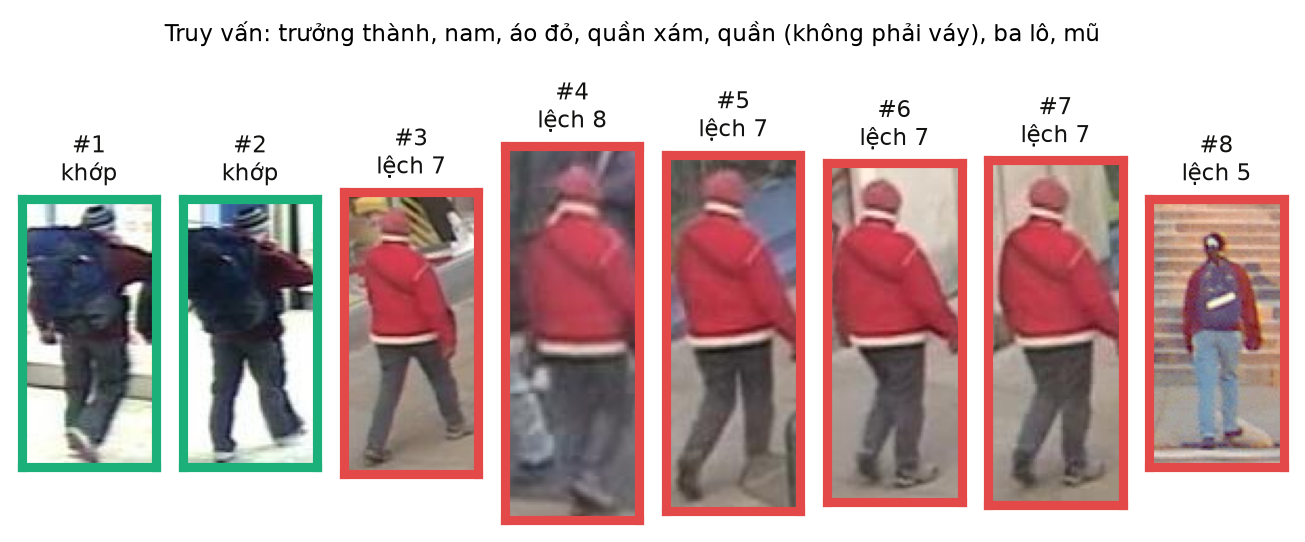
\includegraphics[width=0.9\linewidth]{example.png}
\caption{Một query thật trên gallery PETA và 8 ảnh đứng đầu, xếp bằng mô hình ViT-L được huấn luyện không có PETA. Viền xanh là ảnh khớp chính xác cả 40 thuộc tính. Viền đỏ là ảnh lệch nhiều thuộc tính. Các ảnh lệch 7 thuộc tính trông gần giống mô tả của query, nhưng label của chúng khác query ở 7 trong 40 thuộc tính.}
\label{fig:example}
\end{figure}

Một ảnh gallery được coi là \textbf{khớp chính xác} với query khi vector label (tạm dịch: nhãn) của nó bằng query ở cả 40 vị trí. Theo cách ban tổ chức tạo dữ liệu, mỗi vector label khác nhau có mặt trong gallery trở thành một query. Trên tập val có 3462 query, và mỗi query có ít nhất một ảnh khớp chính xác.

\subsection{Dữ liệu và camera mới}

Dữ liệu giống Track 1, gồm ảnh của ba bộ dữ liệu PA100k~\cite{pa100k}, Market1501~\cite{market} và PETA~\cite{peta}, mỗi bộ chụp bằng một hệ thống camera riêng. Mỗi bộ như vậy là một \textbf{domain} (tạm dịch: miền dữ liệu). Bài nộp được chấm trên gallery của một domain camera thứ tư, không có trong dữ liệu huấn luyện. Đây là điểm khó chính của cuộc thi.

Ba gallery val có cấu trúc khác nhau. Ở PETA, 61\% query chỉ có đúng một ảnh khớp. Tỉ lệ này là 42\% ở PA100k và 15\% ở Market1501, nơi một query có trung vị 10 ảnh khớp. Vì vậy điểm của cùng một mô hình khác nhau nhiều giữa ba gallery, và khi so hai mô hình, chúng tôi luôn so trên cùng một gallery.

\subsection{Cách chấm điểm}
\label{sec:metric}

\paragraph{Vấn đề với mAP.} Chỉ số quen thuộc của bài toán truy xuất là mAP. mAP chỉ quan tâm vị trí của các ảnh khớp chính xác. Một ảnh lệch một thuộc tính bị coi sai giống hệt một ảnh lệch 20 thuộc tính. Trong ứng dụng thật, người dùng vẫn được lợi khi các ảnh gần đúng đứng trước các ảnh hoàn toàn sai, vì label của từng thuộc tính vốn không hoàn hảo.

\paragraph{mADM.} Cuộc thi dùng \textbf{mADM} (mean average degree of match), một biến thể của mAP cộng điểm cho các ảnh khớp gần. Với query $q$ và ảnh $g$, gọi $\mathrm{dom}(q,g)$ là tỉ lệ thuộc tính bằng nhau giữa $q$ và label của $g$. Mức khớp được chuẩn hoá theo chính gallery của query đó:
\begin{equation}
\ndom(q,g)=\max\!\left(0,\ \frac{\mathrm{dom}(q,g)-\overline{\mathrm{dom}}_q}{\max_{g'}\mathrm{dom}(q,g')-\overline{\mathrm{dom}}_q}\right),
\end{equation}
với $\overline{\mathrm{dom}}_q$ là trung bình của dom trên toàn gallery. Ảnh khớp chính xác có $\ndom=1$. Ảnh có mức khớp dưới trung bình có $\ndom=0$. Gọi $r_1<\dots<r_R$ là vị trí của $R$ ảnh khớp chính xác trong danh sách trả về. Điểm của một query và chỉ số tổng là
\begin{equation}
\mathrm{ADM}(q)=\frac{1}{R}\sum_{m=1}^{R}\frac{1}{r_m}\sum_{j=1}^{r_m}\ndom(q,g_{(j)}), \qquad \mathrm{mADM}=\frac{1}{|Q|}\sum_{q}\mathrm{ADM}(q),
\end{equation}
với $g_{(j)}$ là ảnh ở vị trí $j$. Công thức có cùng cấu trúc với AP. Khác biệt duy nhất là thay cho việc đếm số ảnh khớp chính xác trong $r_m$ vị trí đầu, công thức cộng ndom của cả $r_m$ ảnh đó.

\paragraph{Một ảnh khớp gần được bao nhiêu điểm.} Trên PETA, dom trung bình của một query khoảng 0.82, và ảnh tốt nhất luôn khớp chính xác. Một ảnh lệch $j$ thuộc tính có $\mathrm{dom}=1-j/40$, nên
\begin{equation}
\ndom(j)\approx\frac{1-j/40-0.82}{1-0.82}=1-\frac{j}{7.2}.
\end{equation}
Hình~\ref{fig:ndom} cho thấy ảnh lệch 1 thuộc tính nhận 0.86 điểm, ảnh lệch 2 nhận 0.72, và ảnh lệch từ 8 thuộc tính trở lên không nhận điểm nào.

\begin{figure}[H]
\centering
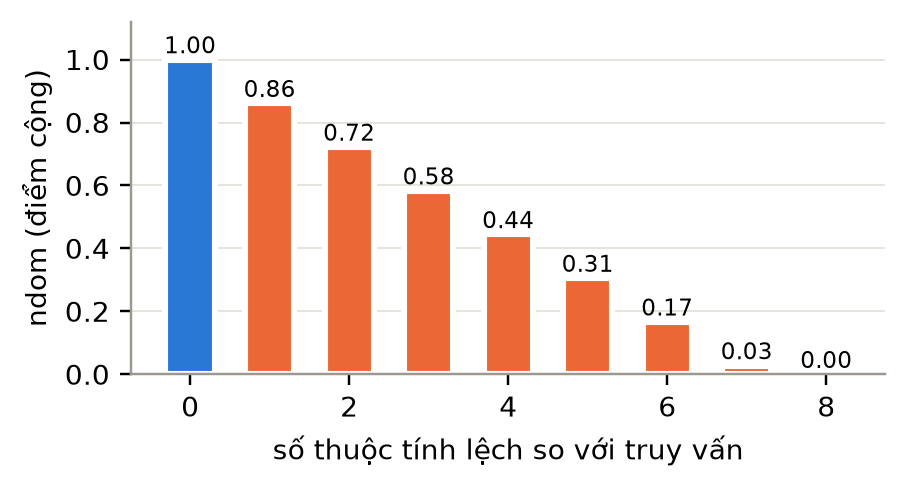
\includegraphics[width=0.5\linewidth]{ndom.png}
\caption{Điểm ndom mà một ảnh nhận được theo số thuộc tính lệch so với query, ở dom trung bình 0.82 của PETA. Ảnh lệch 1 đến 2 thuộc tính vẫn nhận 72 đến 86\% điểm của một ảnh khớp chính xác.}
\label{fig:ndom}
\end{figure}

\paragraph{mADM thưởng gì.} Mỗi ảnh ảnh hưởng tới ADM theo hai đường. Nếu ảnh khớp chính xác, vị trí của nó là một $r_m$ và quyết định hệ số $1/r_m$. Nếu ảnh đứng trước một ảnh khớp chính xác, ndom của nó được cộng vào tổng. Một hàm xếp hạng tốt vì vậy phải làm hai việc. Nó phải đưa ảnh khớp chính xác lên thật cao, và các ảnh đứng trước ảnh khớp phải lệch ít thuộc tính.

\subsection{Ràng buộc khi chạy}

Bài nộp là một chương trình chạy trên máy chấm có 6 luồng CPU, không GPU, không mạng, với giới hạn 3600 giây. Chương trình nhận toàn bộ query và toàn bộ ảnh gallery, rồi trả về một ma trận điểm có kích thước số query nhân số ảnh. Phần tốn thời gian là tính 40 xác suất cho mỗi ảnh gallery bằng mô hình nhận dạng thuộc tính. Ràng buộc này chỉ cho phép một mô hình cỡ ViT-B chạy an toàn (mục~\ref{sec:lb}).

\begin{ghichu}
mADM có cấu trúc của AP, nhưng tại mỗi ảnh khớp chính xác, nó đo mức khớp trung bình của cả phần danh sách đứng trước. Một hàm xếp hạng tốt phải đưa lên đầu những ảnh đúng ở gần như mọi thuộc tính, nên cả 40 xác suất thành phần đều phải có chất lượng tốt trên camera mới.
\end{ghichu}

%=====================================================================
\section{Từ 40 xác suất tới một thứ hạng}
\label{sec:score}

\subsection{Mô hình cho ra gì}

Hệ thống gồm hai phần. Phần thứ nhất là một mô hình nhận dạng thuộc tính, giống Track 1. Mô hình gồm một \textbf{backbone} (tạm dịch: bộ trích đặc trưng) DINOv3 ViT-B/16~\cite{dinov3} nhận ảnh 256×128 và một query head (tạm dịch: head truy vấn) với một vector query riêng cho mỗi thuộc tính. Với mỗi ảnh gallery $g$, mô hình trả về 40 số thực gọi là \textbf{logit} $z_{gk}$, và hàm sigmoid đổi chúng thành 40 xác suất $p_{gk}=1/(1+e^{-z_{gk}})$. Phần thứ hai là một \textbf{hàm xếp hạng} $s(q,g)$, biến query và 40 xác suất thành một con số. Gallery được xếp theo con số này giảm dần. Mục này bàn về phần thứ hai, vì đó là chỗ quyết định những tính chất nào của xác suất là quan trọng.

\subsection{Khoảng cách L1 của baseline và chỗ nó hỏng}

Baseline của ban tổ chức dùng
\begin{equation}
s_{L1}(q,g)=-\sum_{k=1}^{40}|q_k-p_{gk}| .
\end{equation}
Mỗi số hạng $|q_k-p_{gk}|$ là xác suất mô hình cho rằng ảnh lệch query ở thuộc tính $k$. Tổng của chúng là số thuộc tính lệch kỳ vọng. Hàm này đo đúng thành phần thứ hai của mADM, là mức khớp gần, nhưng không đo xác suất ảnh khớp chính xác.

Xét ba ảnh. Ảnh A có 40 xác suất đều bằng 0.9 về phía query. Số thuộc tính lệch kỳ vọng của A là 4, và xác suất A khớp chính xác là $0.9^{40}\approx0.015$. Ảnh B có 39 xác suất bằng 1 về phía query và một xác suất bằng 0.5. Số lệch kỳ vọng của B là 0.5, và xác suất khớp chính xác là 0.5. L1 xếp B trên A, đúng như mong muốn. Ảnh C có 36 thuộc tính chắc chắn đúng và 4 thuộc tính chắc chắn sai. Số lệch kỳ vọng của C là 4, bằng A, dù xác suất C khớp chính xác bằng 0. L1 không phân biệt được A với C.

\subsection{Xếp theo log-likelihood của đúng vector query}

\paragraph{Yêu cầu.} Hàm xếp hạng cần tăng theo xác suất ảnh có đúng vector query. Nguyên lý xếp hạng theo xác suất~\cite{prp} cho biết xếp theo xác suất liên quan giảm dần cho số ảnh liên quan kỳ vọng lớn nhất ở mọi độ sâu của danh sách, khi các xác suất đó đúng. Với mADM, một ảnh có xác suất khớp chính xác cao cũng có xác suất cao chỉ lệch ít thuộc tính, nên cùng một hàm phục vụ được cả hai thành phần.

\paragraph{Cơ chế.} Giả sử khi đã biết ảnh, 40 thuộc tính độc lập với nhau. Xác suất ảnh $g$ có đúng vector $q$ là tích của 40 xác suất thành phần. Lấy log của tích này, ta được \textbf{log-likelihood} (tạm dịch: log hợp lý) của vector query:
\begin{equation}
s_{LL}(q,g)=\sum_{k=1}^{40}\Big[q_k\log p_{gk}+(1-q_k)\log(1-p_{gk})\Big].
\label{eq:ll}
\end{equation}
Mỗi số hạng là log của xác suất mà mô hình gán cho đúng giá trị của query ở thuộc tính $k$. Số hạng bằng 0 khi mô hình chắc chắn đồng ý với query, và rất âm khi mô hình chắc chắn phản đối. Xác suất được kẹp trong $[10^{-4},1-10^{-4}]$ để tránh log của 0. Phụ lục~\ref{app:algo} cho thấy ma trận điểm của mọi cặp query và ảnh tính được bằng một phép nhân ma trận, nên bước chấm điểm gần như không tốn thời gian so với backbone.

Hình~\ref{fig:pipeline} cho thấy công thức này làm việc trên một query thật. Mỗi hàng là một ảnh gallery, và 40 ô của hàng là 40 số hạng của phương trình~\eqref{eq:ll}. Điểm của ảnh là tổng của 40 ô. Ảnh khớp chính xác duy nhất của query này chỉ đứng hạng 13. Lý do nằm ở đúng một ô. Label của ảnh, giống query, không đánh dấu nhóm tuổi nào, nhưng mô hình chắc chắn đây là người trưởng thành và gán cho giá trị 0 của query xác suất $e^{-3.5}\approx0.03$. Ô đó trừ 3.5 vào tổng, đủ đẩy ảnh xuống dưới 12 ảnh lệch một hoặc hai thuộc tính. Ở hàng cuối, một ảnh lệch 5 thuộc tính nhận 5 ô đậm và tụt xuống hạng 3482.

\begin{figure}[H]
\centering
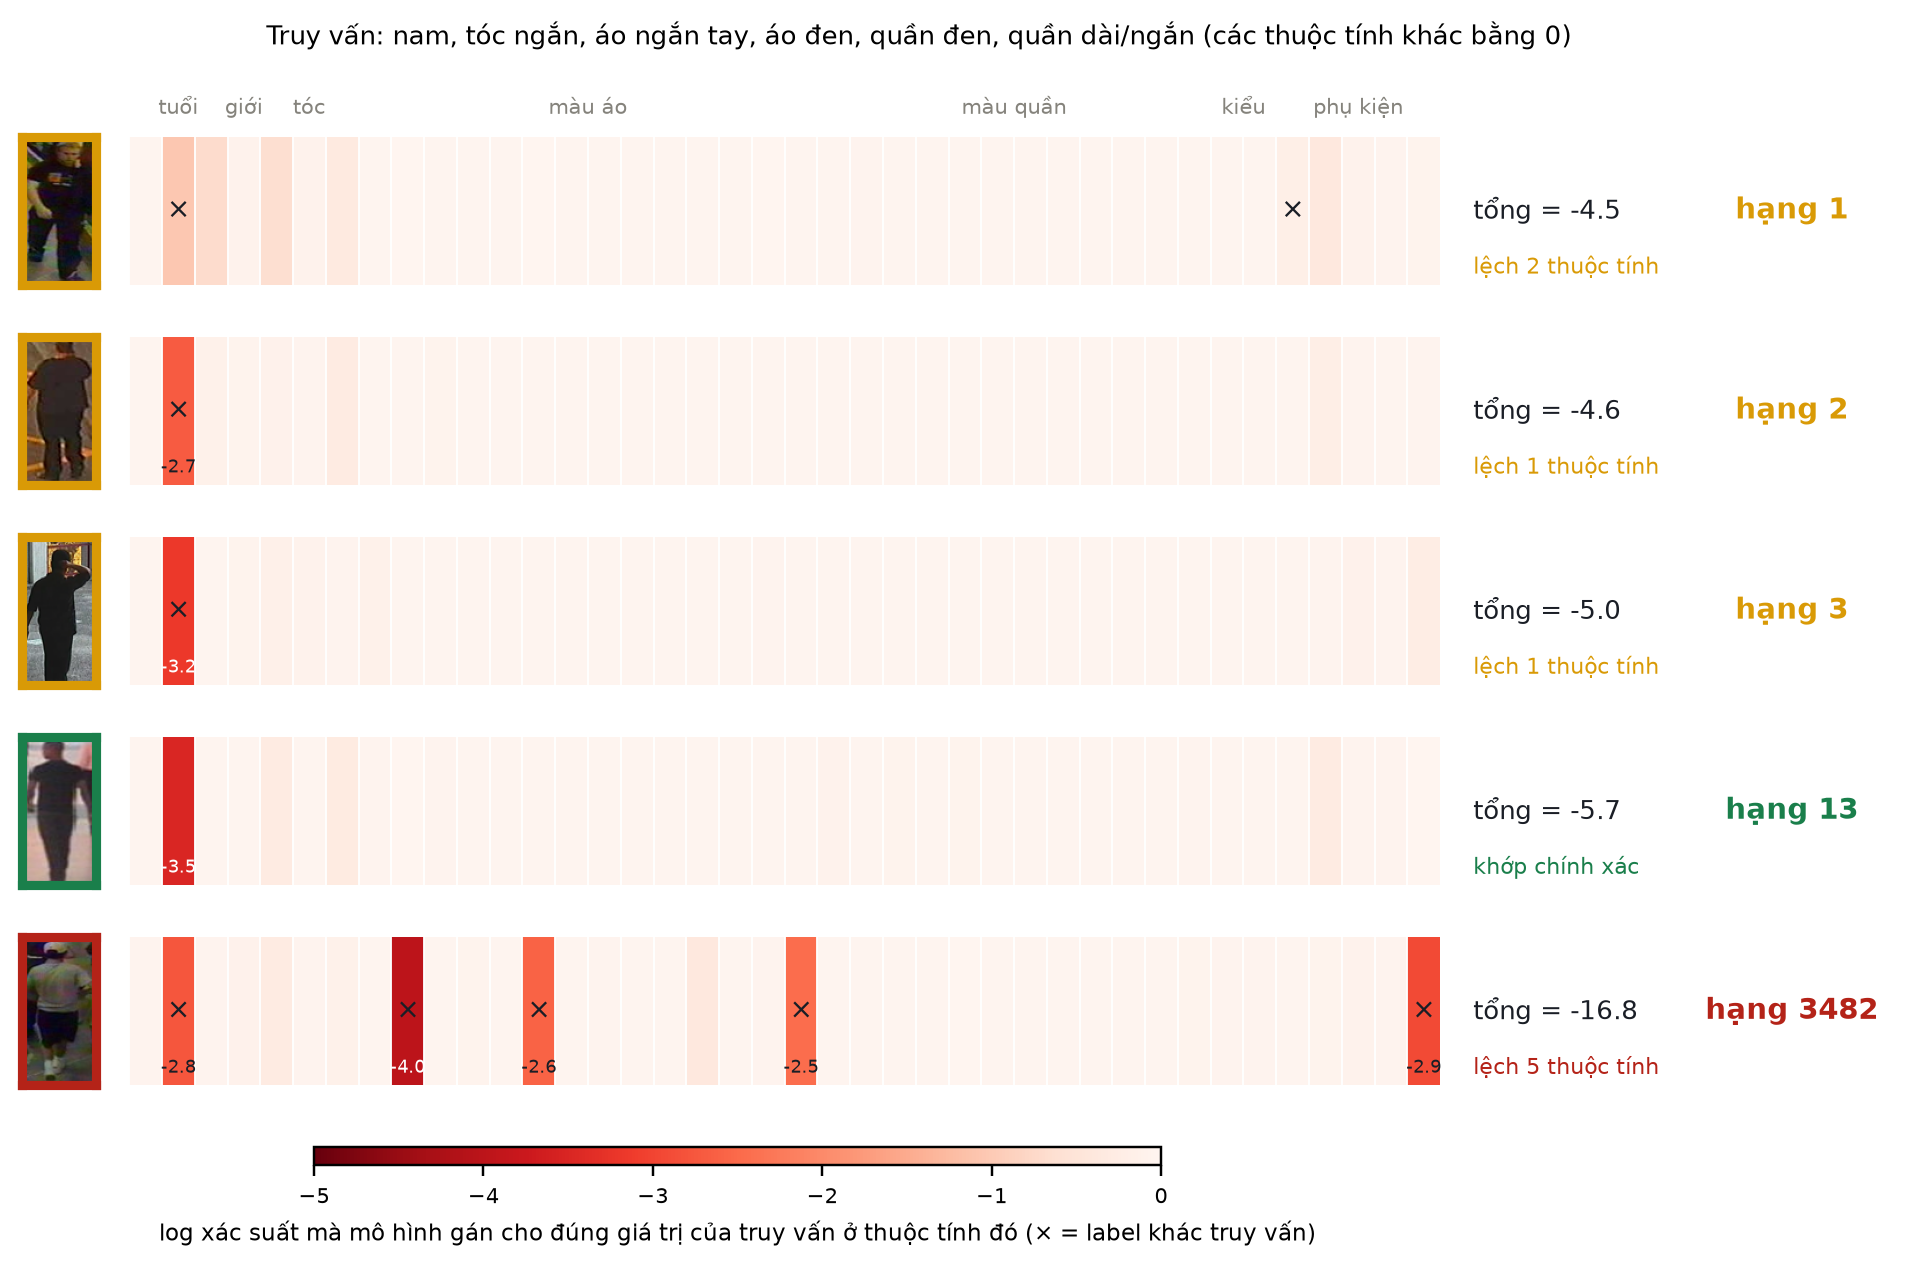
\includegraphics[width=\linewidth]{t2_pipeline.png}
\caption{Điểm log-likelihood của năm ảnh PETA cho cùng một query, tính bằng mô hình ViT-L được huấn luyện không có PETA. Mỗi ô là log xác suất mà mô hình gán cho đúng giá trị của query ở một thuộc tính, ô càng đậm càng bị phạt nặng, và dấu × đánh dấu thuộc tính mà label của ảnh khác query. Điểm của ảnh là tổng 40 ô. Ảnh khớp chính xác (viền xanh) bị một ô ở thuộc tính trưởng thành đẩy xuống hạng 13. Ảnh lệch 5 thuộc tính (viền đỏ) có 5 ô đậm và đứng hạng 3482 trên 6963 ảnh.}
\label{fig:pipeline}
\end{figure}

\paragraph{Kết quả.} Hình~\ref{fig:l1ll} so hai hàm trên cùng gallery và cùng xác suất. Với query này, L1 đặt ảnh khớp chính xác đầu tiên ở hạng 47, còn log-likelihood đặt nó ở hạng 1. Sáu ảnh đứng đầu theo L1 đều là nữ theo label, trong khi query là nam, và mô hình cũng nhận ra điều đó với xác suất cao. Số lệch kỳ vọng của chúng chỉ khoảng 5.1 đến 5.4, vì ngoài giới tính, màu áo và kính râm, mô hình chắc chắn ở mọi thuộc tính khác. Hai ảnh khớp chính xác có số lệch kỳ vọng 6.0 và 6.7, cao hơn, vì mô hình hơi không chắc ở nhiều thuộc tính cùng lúc. L1 cộng các nghi ngờ nhỏ này lại và đẩy ảnh khớp xuống. Log-likelihood thì phạt nặng mỗi thuộc tính bị phản đối mạnh, nên đưa hai ảnh khớp lên hạng 1 và 3.

\begin{figure}[H]
\centering
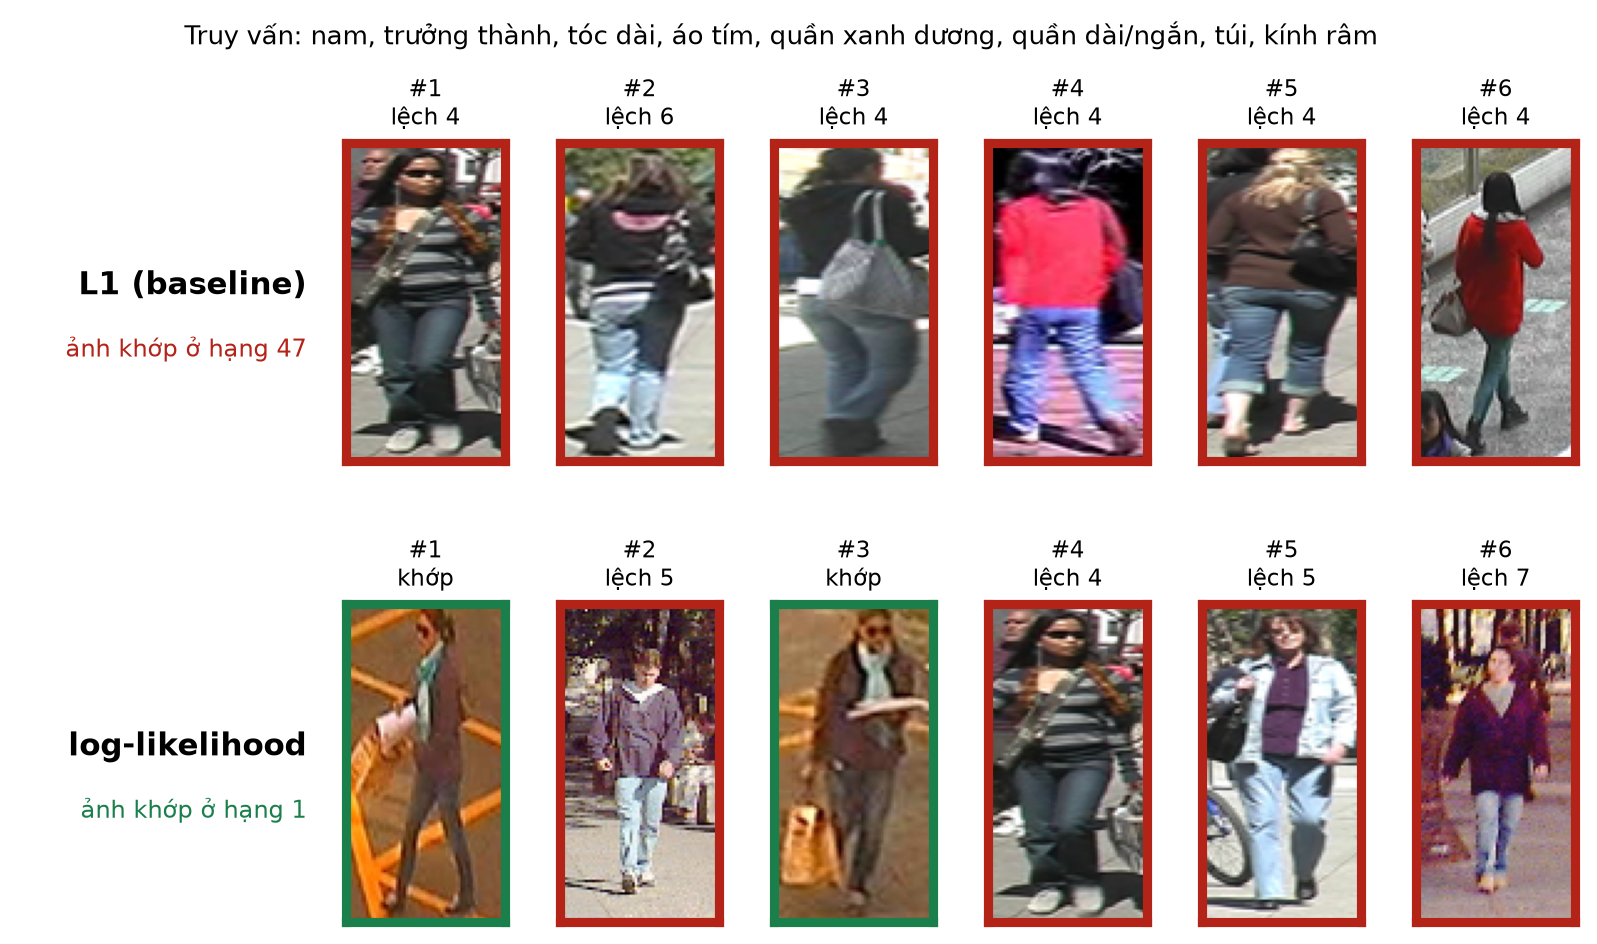
\includegraphics[width=0.85\linewidth]{t2_l1_vs_ll.png}
\caption{Cùng một query và cùng xác suất của mô hình, xếp theo L1 (hàng trên) và theo log-likelihood (hàng dưới). Viền xanh là ảnh khớp chính xác, viền đỏ là ảnh lệch từ 3 thuộc tính trở lên. L1 đưa lên đầu các ảnh lệch 4 đến 6 thuộc tính và để ảnh khớp đầu tiên ở hạng 47.}
\label{fig:l1ll}
\end{figure}

Bảng~\ref{tab:llvsl1} cho thấy ưu thế này lặp lại trên bốn mô hình và ở cả sáu chỉ số xếp hạng. Trên toàn bộ 48 lần huấn luyện có lưu logit, mức tăng mADM là 0.052 trung bình trên PETA (0.037 đến 0.064, 41 lần chạy), 0.049 trên Market1501 (0.046 đến 0.054, 5 lần chạy) và 0.086 trên PA100k (0.082 đến 0.091, 2 lần chạy). Mức chênh này lớn hơn mọi khác biệt giữa các mô hình mà chúng tôi đo sau đó, nên phần còn lại của báo cáo dùng $s_{LL}$.

\begin{table}[H]
\centering\small
\begin{tabular}{@{}llcccccc@{}}
\toprule
Mô hình (PETA giấu) & Hàm & mADM & mAP & mINP & R-1 & R-5 & R-10 \\
\midrule
ViT-B query head & L1 & 0.5798 & 0.1998 & 0.1511 & 0.1798 & 0.3460 & 0.4192 \\
 & $s_{LL}$ & 0.6270 & 0.2789 & 0.2184 & 0.2422 & 0.4640 & 0.5525 \\
ViT-B query head + group CE & L1 & 0.5896 & 0.2040 & 0.1524 & 0.1809 & 0.3562 & 0.4419 \\
 & $s_{LL}$ & 0.6406 & 0.2980 & 0.2349 & 0.2626 & 0.4889 & 0.5876 \\
ViT-L, distillation DINOv3-L + CLIP-L & L1 & 0.6053 & 0.2169 & 0.1649 & 0.1985 & 0.3738 & 0.4515 \\
 & $s_{LL}$ & 0.6635 & 0.3175 & 0.2559 & 0.2813 & 0.5139 & 0.5967 \\
ViT-L, distillation DINOv3-L + MetaCLIP2-H & L1 & 0.6057 & 0.2144 & 0.1642 & 0.1940 & 0.3698 & 0.4509 \\
 & $s_{LL}$ & 0.6697 & 0.3231 & 0.2607 & 0.2881 & 0.5184 & 0.6058 \\
\bottomrule
\end{tabular}
\caption{L1 so với log-likelihood trên bốn mô hình, gallery PETA giấu (1763 query). Log-likelihood thắng ở mọi chỉ số, với mADM cao hơn 0.047 đến 0.064 và Rank-1 cao hơn 0.06 đến 0.09.}
\label{tab:llvsl1}
\end{table}

\subsection{Hệ quả: độ lớn của xác suất quyết định thứ hạng}

Ở Track 1, mỗi xác suất chỉ được so với threshold (tạm dịch: ngưỡng) 0.5, nên xác suất 0.6 hay 0.99 cho cùng một câu trả lời. Ở Track 2, phương trình~\eqref{eq:ll} dùng chính độ lớn của xác suất. Một thuộc tính bị đoán sai với xác suất 0.999 đóng góp $\log 0.001\approx-6.9$ vào điểm, bằng tổng phạt của khoảng 20 thuộc tính hơi không chắc. Câu hỏi tự nhiên tiếp theo là xác suất của mô hình có đúng độ lớn hay không, nhất là trên camera mới. Đây chính là câu hỏi về calibration.

\begin{ghichu}
Log-likelihood của đúng vector query xếp ảnh theo xác suất khớp chính xác, và thắng L1 với khoảng cách lớn hơn mọi thay đổi mô hình. Cái giá của nó là mỗi thuộc tính bị đoán sai một cách tự tin có thể đẩy một ảnh khớp chính xác ra khỏi phần đầu danh sách. Độ lớn của từng xác suất vì vậy trở thành thứ quyết định thứ hạng.
\end{ghichu}

%=====================================================================
\section{Calibration trên camera mới}
\label{sec:calib}

\subsection{Calibration là gì}

\paragraph{Định nghĩa.} Một mô hình được \textbf{calibrated} (tạm dịch: hiệu chỉnh tốt) khi trong mọi nhóm ảnh mà mô hình gán xác suất khoảng 0.7 cho một thuộc tính, khoảng 70\% số ảnh thật sự có thuộc tính đó. Khi tần suất thật khác xác suất mô hình nói, mô hình bị \textbf{miscalibrated} (tạm dịch: sai lệch hiệu chỉnh). Mô hình quá tự tin khi xác suất 0.95 chỉ đúng 80\% số lần, và thiếu tự tin khi xác suất 0.6 đúng 90\% số lần.

\paragraph{Cách nhìn.} Cách trực quan nhất là \textbf{reliability diagram} (tạm dịch: biểu đồ độ tin cậy). Ta chia các ô (ảnh, thuộc tính) theo xác suất mô hình trả về, rồi vẽ tần suất label dương thật của mỗi nhóm theo xác suất trung bình của nhóm. Mô hình hiệu chỉnh tốt nằm trên đường chéo. Hình~\ref{fig:rel} vẽ biểu đồ này cho hai mô hình, trên val của hai camera nguồn và trên PETA giấu.

\begin{figure}[H]
\centering
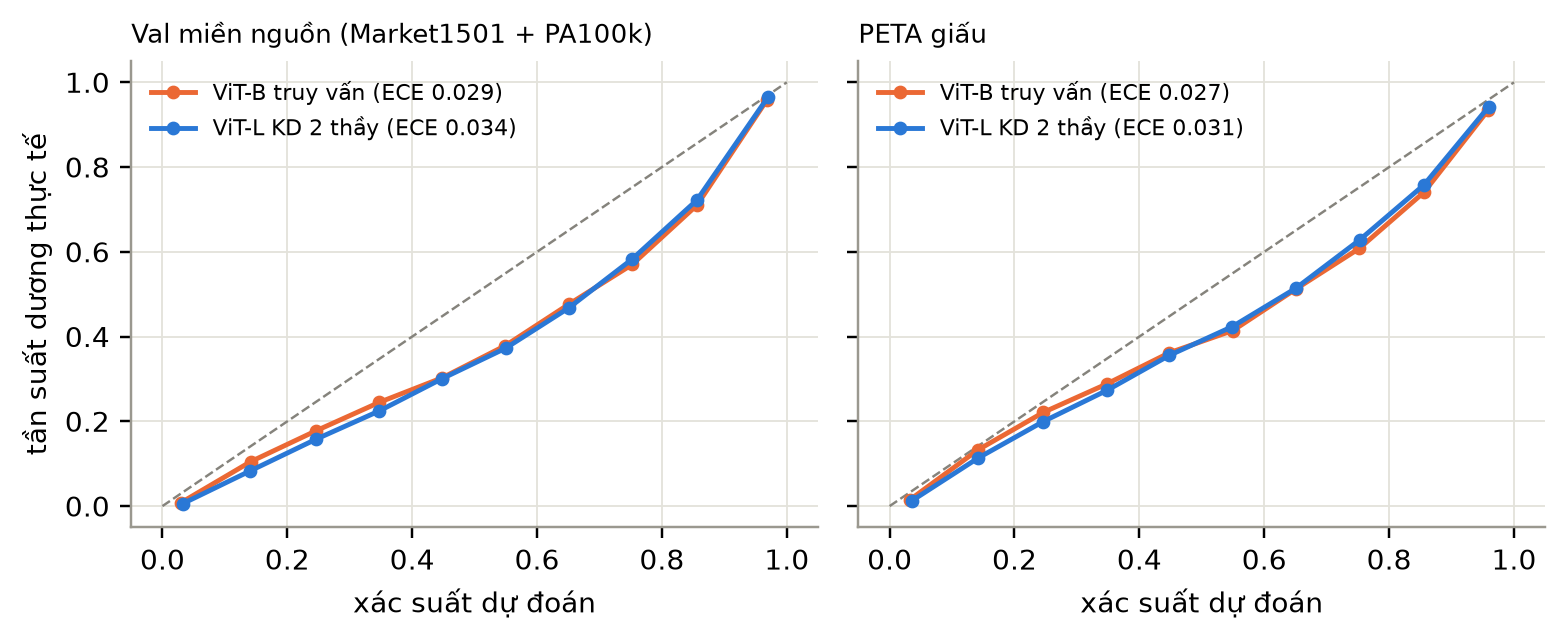
\includegraphics[width=\linewidth]{reliability.png}
\caption{Reliability diagram gộp 40 thuộc tính trên val của hai camera nguồn (trái) và trên PETA giấu (phải). Cả hai mô hình dự đoán dương nhiều hơn thực tế ở vùng xác suất trung gian, theo cùng một kiểu trên cả hai domain. Biểu đồ gộp có thể che các sai lệch ngược dấu giữa các thuộc tính, nên các mục sau đo theo từng thuộc tính.}
\label{fig:rel}
\end{figure}

\paragraph{Sửa calibration sau huấn luyện.} Cách sửa phổ biến là \textbf{Platt scaling}. Với mỗi thuộc tính $k$, ta học hai số $a_k$ và $b_k$, rồi thay xác suất bằng $\sigma(a_k z_k+b_k)$. Hệ số dốc $a_k$ làm xác suất sắc hơn khi lớn hơn 1, hoặc mềm hơn khi nhỏ hơn 1. Hệ số chặn $b_k$ dời toàn bộ xác suất của thuộc tính đó lên hoặc xuống. Phép biến đổi này đồng biến, nên không đổi thứ tự các ảnh ở từng thuộc tính. Nó chỉ đổi độ lớn của xác suất. Khi $a_k$ bằng nhau cho mọi thuộc tính và $b_k=0$, phép biến đổi trở thành \textbf{temperature scaling} (tạm dịch: hiệu chỉnh nhiệt độ) với $T=1/a$~\cite{guo}.

\paragraph{Đo bằng NLL.} Để đo chất lượng xác suất bằng một con số, chúng tôi dùng \textbf{NLL trên một ảnh}, là trung bình trên các ảnh của $-\sum_k[y_k\log p_k+(1-y_k)\log(1-p_k)]$, với $y$ là vector label thật. Đại lượng này chính là $-s_{LL}$ của phương trình~\eqref{eq:ll} khi query bằng label của ảnh. Nó đo xem mô hình phạt ảnh khớp chính xác nặng tới đâu, và đơn vị của nó là nats. Theo Kull và Flach~\cite{kull}, NLL tách được thành hai phần. Phần \textbf{calibration} là lượng NLL mà Platt scaling theo từng thuộc tính, học trên chính các label đó, loại bỏ được. Phần \textbf{refinement} (tạm dịch: độ phân tách) là lượng NLL còn lại, phụ thuộc vào việc mô hình tách ảnh có và không có thuộc tính tốt đến đâu. Nhận định của ban tổ chức, viết theo ngôn ngữ này, là phần calibration trên camera mới lớn và là nút thắt của truy xuất.

\subsection{Sai lệch có thật}

Để đo giới hạn trên của việc sửa calibration, chúng tôi học Platt scaling trên chính label của PETA giấu rồi chấm mADM trên PETA. Phép sửa này dùng label của camera chấm nên không làm được trong thực tế. Ta gọi nó là \textbf{oracle}. Bảng~\ref{tab:calib} cho thấy oracle lấy lại 0.026 mADM trên PETA, 0.018 trên Market1501 và 0.057 trên PA100k, nhiều hơn mọi thay đổi mô hình ở mục~\ref{sec:train}. Ban tổ chức đúng khi cho rằng chất lượng xác suất giới hạn truy xuất.

\begin{table}[H]
\centering\small
\begin{tabular}{@{}lccc@{}}
\toprule
Bộ giấu & PETA & Market1501 & PA100k \\
\midrule
số lần huấn luyện & 41 & 5 & 2 \\
NLL trên camera giấu (nats) & 6.97 & 6.09 & 9.38 \\
phần calibration, camera giấu & 1.29 & 1.10 & 3.88 \\
phần calibration, val của camera nguồn & 1.10 & 0.89 & 3.74 \\
\midrule
thay đổi mADM, Platt oracle & +0.0264 & +0.0175 & +0.0573 \\
thay đổi mADM, Platt học trên nguồn & $-$0.0086 & $-$0.0053 & +0.0363 \\
số lần huấn luyện mà Platt trên nguồn có ích & 0/41 & 0/5 & 1/2 \\
\midrule
NLL sau Platt, $a_k$ nguồn và $b_k$ nguồn & 6.60 & 5.87 & 6.10 \\
\phantom{NLL sau Platt,} $a_k$ nguồn và $b_k$ camera giấu & 6.18 & 5.12 & 5.88 \\
\phantom{NLL sau Platt,} $a_k$ camera giấu và $b_k$ nguồn & 6.55 & 5.85 & 8.19 \\
\phantom{NLL sau Platt,} $a_k$ và $b_k$ camera giấu (oracle) & 5.68 & 4.99 & 5.51 \\
\bottomrule
\end{tabular}
\caption{Calibration trên camera giấu và trên camera nguồn, trung bình trên các lần huấn luyện. Oracle lấy lại nhiều mADM, nhưng Platt học trên nguồn làm mADM giảm. Hoán đổi hai tham số cho thấy hệ số chặn $b_k$ là phần không chuyển được.}
\label{tab:calib}
\end{table}

\subsection{Nhưng phần lớn không do camera mới gây ra}

Nếu camera mới là nguyên nhân, phần calibration trên camera nguồn phải nhỏ. Bảng~\ref{tab:calib} cho thấy điều ngược lại. Trên val của chính hai camera nguồn, phần calibration đã là 1.10 nats ở fold PETA, so với 1.29 trên PETA. Phần trên camera giấu lớn hơn ở 44 trên 48 lần huấn luyện, nhưng phần vượt chỉ chiếm 3 đến 19\% tổng. Phần lớn sai lệch có sẵn từ cách huấn luyện. Mục tiêu huấn luyện được làm mềm về 0.025 và 0.975, và loss được đánh weight (tạm dịch: trọng số) theo tần suất thuộc tính (mục~\ref{sec:smooth}). Mạng vì vậy không được huấn luyện để trả về đúng tần suất, ở bất kỳ camera nào.

\subsection{Và phần khác nhau thì không chuyển được}

\paragraph{Phép thử.} Nếu sai lệch gần giống nhau ở hai domain, Platt học trên val của camera nguồn sẽ sửa được phần lớn sai lệch trên camera mới. Phép này đúng là làm giảm NLL trên PETA, từ 6.97 xuống 6.60. Nhưng nó làm mADM giảm ở 47 trên 48 lần huấn luyện. Ngoại lệ duy nhất là mô hình head tuyến tính giấu PA100k, mô hình có calibration kém nhất.

\paragraph{Định vị chỗ hỏng.} Khối cuối của Bảng~\ref{tab:calib} hoán đổi hai tham số. Dùng hệ số dốc học trên nguồn với hệ số chặn học trên camera giấu lấy lại 61\% mức giảm NLL của oracle trên PETA, 88\% trên Market1501 và 90\% trên PA100k. Làm ngược lại, dùng hệ số dốc của camera giấu với hệ số chặn của nguồn, chỉ lấy lại 33\%, 22\% và 31\%. Hệ số dốc chuyển được giữa các camera. Hệ số chặn của từng thuộc tính thì không.

Hình~\ref{fig:calibattr} cho thấy điều này ở từng thuộc tính. Ba ô bên trái là ba thuộc tính có hệ số dốc gần như không đổi giữa hai domain nhưng hệ số chặn dời nhiều nhất. Ở thuộc tính áo trắng, hệ số dốc là 1.13 trên nguồn và 1.25 trên PETA, nhưng hệ số chặn đổi từ $-1.17$ sang $+1.23$. Đường cong Platt học trên nguồn có cùng độ dốc với đường cong oracle nhưng nằm lệch hẳn sang phải, nên nó kéo xác suất áo trắng xuống thấp đúng lúc PETA cần kéo lên. Hai ô bên phải gộp 32 thuộc tính. Hệ số dốc nằm quanh đường chéo với độ lệch trung vị 0.19, còn hệ số chặn lệch trung vị 0.76.

\begin{figure}[H]
\centering
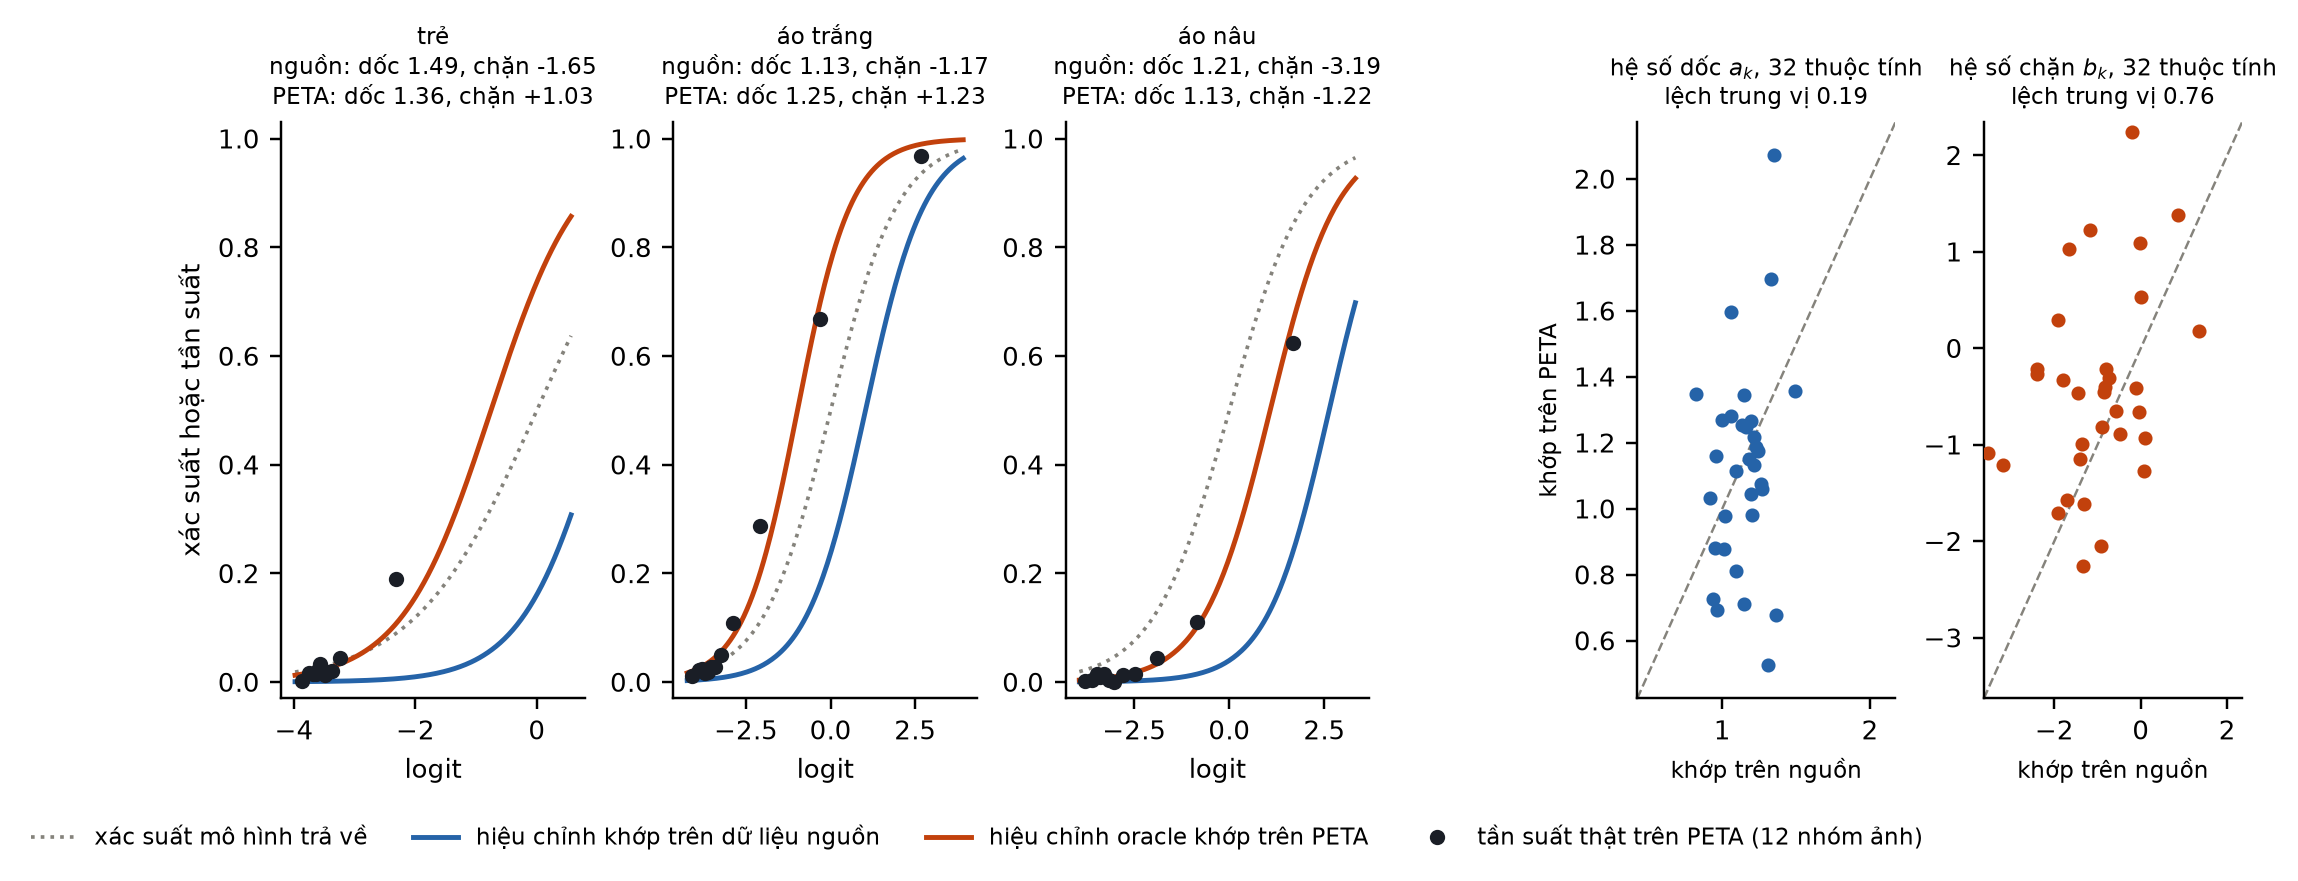
\includegraphics[width=\linewidth]{t2_calib_attr.png}
\caption{Platt scaling theo từng thuộc tính, mô hình ViT-L huấn luyện không có PETA. Ba ô trái là ba thuộc tính có hệ số dốc ổn định nhất và hệ số chặn dời xa nhất. Chấm đen là tần suất label dương thật trên PETA trong 12 nhóm ảnh xếp theo logit. Đường xanh là Platt học trên val của hai camera nguồn, đường cam là Platt học trên PETA. Hai ô phải so hệ số học trên nguồn với hệ số học trên PETA, cho 32 thuộc tính có đủ ảnh dương ở cả hai phía. Hệ số dốc chuyển được, hệ số chặn thì không.}
\label{fig:calibattr}
\end{figure}

Kết quả này giống kết quả Track 1, nơi offset threshold khớp trên camera nguồn không chuyển sang camera mới. Hệ số chặn của Platt và offset threshold là cùng một thứ, một lượng dời logit riêng cho từng thuộc tính. Lượng dời này phụ thuộc vào tần suất thuộc tính và vào annotation convention (tạm dịch: quy ước gán nhãn) của từng camera, và cả hai đều thay đổi khi đổi camera.

\subsection{Vì sao NLL giảm mà mADM lại giảm}

NLL đo xác suất của vector label của chính từng ảnh. Thứ hạng thì phụ thuộc vào xác suất đó so với xác suất của các ảnh cạnh tranh. Một hệ số chặn sai domain dời điểm của mọi ảnh trong gallery ở thuộc tính đó. Ví dụ, nếu Platt kéo xác suất áo trắng xuống, mọi ảnh áo trắng đều bị phạt thêm khi query có áo trắng, kể cả ảnh khớp chính xác. Các ảnh áo xám mà mô hình nhầm sang áo trắng lại được lợi khi query có áo xám. Thứ tự giữa ảnh khớp và ảnh cạnh tranh có thể đảo ngay cả khi NLL trung bình giảm.

\subsection{Các tinh chỉnh khác ở bước chấm điểm}
\label{sec:robust}

Một câu hỏi còn lại là một temperature chung $T>1$, hoặc weight theo độ tin cậy của từng thuộc tính như Specker và Beyerer đề xuất~\cite{specker21}, có giúp ổn định trên mọi camera giấu hay không. Chúng tôi áp $T\in\{1.0,1.1,1.2,1.3,1.4\}$ lên logit của 5 mô hình trên ba camera giấu, và thử weight $w_k=2(\mathrm{AUC}_k-0.5)$ hoặc bình phương của nó, với AUC đo trên val của camera nguồn.

\begin{figure}[H]
\centering
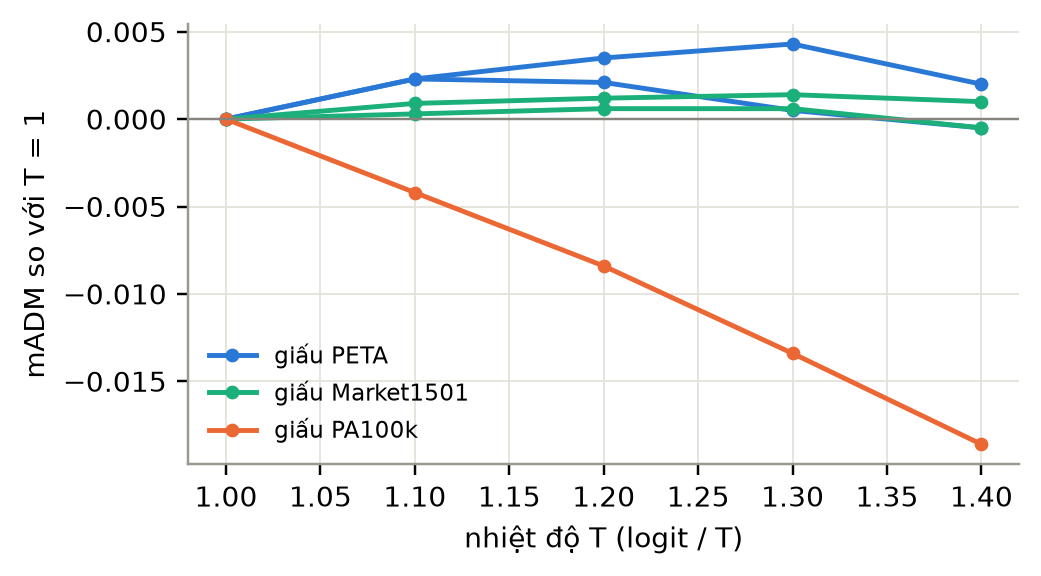
\includegraphics[width=0.6\linewidth]{temperature.png}
\caption{Thay đổi mADM theo temperature trên ba camera giấu. Làm mềm xác suất giúp nhẹ trên PETA và Market1501 nhưng làm giảm mạnh trên PA100k, nên không temperature nào cải thiện ổn định.}
\label{fig:temp}
\end{figure}

\begin{table}[H]
\centering\small
\begin{tabular}{@{}lccc@{}}
\toprule
Thay đổi so với $s_{LL}$ gốc & giấu PETA & giấu Market1501 & giấu PA100k \\
\midrule
temperature $T=1.1$ & +0.002 & +0.0003 đến +0.0009 & $-0.004$ \\
temperature $T=1.3$ & +0.0005 đến +0.004 & +0.0006 đến +0.0014 & $-0.013$ \\
weight $2(\mathrm{AUC}_k-0.5)$ & 0.0000 & +0.0002 & $-0.004$ \\
weight $[2(\mathrm{AUC}_k-0.5)]^2$ & $-0.002$ & $-0.0003$ & $-0.010$ \\
\bottomrule
\end{tabular}
\caption{Thay đổi mADM của các tinh chỉnh ở bước chấm điểm trên ba camera giấu. Không tinh chỉnh nào tăng ở cả ba camera.}
\label{tab:robust}
\end{table}

Hình~\ref{fig:temp} và Bảng~\ref{tab:robust} cho thấy không tinh chỉnh nào cải thiện ở cả ba camera. Kết luận về PA100k chỉ dựa trên một mô hình. Temperature khớp trên val của camera nguồn còn đi ngược hướng. Nó cho $T\approx0.8$, làm xác suất sắc hơn, và làm mADM trên PETA giảm 0.004 đến 0.009. Phụ lục~\ref{app:scores} liệt kê thêm các biến thể của hàm xếp hạng mà chúng tôi đã thử.

\begin{ghichu}
Câu trả lời cho câu hỏi ở tiêu đề là đúng một nửa. Sai lệch calibration có thật và lớn, nhưng phần lớn có sẵn từ cách huấn luyện, và phần riêng của camera mới nằm ở hệ số chặn của từng thuộc tính, thứ mà dữ liệu nguồn không ước lượng được. Mọi phép sửa sau huấn luyện học trên camera nguồn đều mang theo hệ số chặn sai, nên cải thiện phải đến từ bước huấn luyện.
\end{ghichu}

%=====================================================================
\section{Chọn mô hình khi không có ảnh của camera chấm}
\label{sec:proxy}

\subsection{Giấu từng bộ dữ liệu}

Như ở Track 1, điểm trên val cùng domain không dự báo được điểm trên camera mới. Chúng tôi dùng giao thức \textbf{leave-one-dataset-out} (tạm dịch: giấu một bộ dữ liệu). Mô hình học từ train của hai bộ, rồi gallery val của bộ thứ ba được xếp hạng với các query của chính nó. Giấu PETA là phiên bản chính. Giấu Market1501 và giấu PA100k dùng để kiểm tra kết luận có giữ nguyên khi đổi camera hay không. Fold giấu PA100k đặc biệt vì nó chỉ còn 18,7 nghìn ảnh huấn luyện, ít hơn các fold khác khoảng năm lần.

Ba cặp lần huấn luyện chỉ khác seed lệch nhau 0.0008, 0.0016 và 0.0033 mADM, cho độ lệch chuẩn gộp khoảng 0.0015. Sai số chuẩn của hiệu giữa hai mô hình trên cùng các query, tính bằng bootstrap, khoảng 0.0024 đến 0.0029. Chúng tôi chỉ chấp nhận một thay đổi khi hiệu này lớn hơn khoảng hai lần sai số chuẩn và không đổi dấu ở các camera giấu khác.

\subsection{Track 2 cần thước đo khác Track 1}
\label{sec:nll}

\paragraph{Quan sát.} Các mô hình đầu tiên cho Track 2 được chọn bằng tiêu chí của Track 1, là điểm Avg sau khi dời threshold. Tiêu chí đó không thấy lợi ích nào của group CE (mục~\ref{sec:gce}). Ở cặp ViT-B cùng seed, Avg không đổi, trong khi mADM tăng 0.0120.

\paragraph{Giải thích.} Track 1 chỉ quan tâm phía nào của threshold mà xác suất rơi vào, còn Track 2 dùng độ lớn của xác suất. AUC, thước đo ranking của Track 1, chỉ nhìn thứ tự ảnh ở từng thuộc tính. NLL trên camera giấu đo cả thứ tự lẫn độ lớn. Một tiêu chí còn sát mADM hơn là \textbf{log-likelihood listwise}, log của softmax điểm $s_{LL}$ trên toàn gallery, lấy trung bình trên các ảnh khớp chính xác. Tiêu chí này nhìn thấy ảnh khớp đứng cao hay thấp so với các ảnh cạnh tranh.

\begin{figure}[H]
\centering
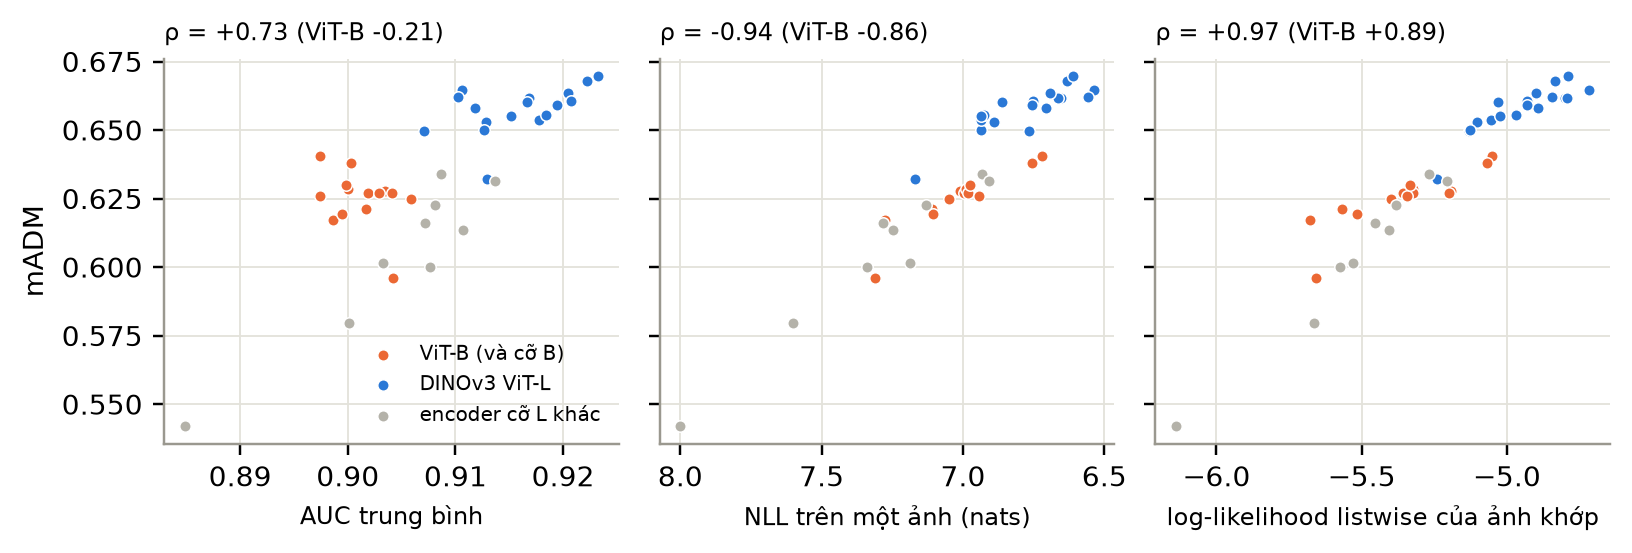
\includegraphics[width=\linewidth]{auc_nll.png}
\caption{mADM theo ba tiêu chí chọn mô hình trên 41 lần huấn luyện giấu PETA. Tiêu đề mỗi ô ghi hệ số Spearman $\rho$ trên mọi lần chạy và trên 14 lần chạy cỡ B. Trục NLL đảo chiều để bên phải luôn là tốt hơn.}
\label{fig:aucnll}
\end{figure}

Hình~\ref{fig:aucnll} kiểm tra ba tiêu chí. Trên mọi lần chạy, mADM bám AUC ở mức vừa (Spearman $\rho=+0.73$), bám NLL chặt ($-0.94$) và bám tiêu chí listwise chặt nhất ($+0.97$). Phần lớn tương quan với AUC đến từ backbone, vì các mô hình ViT-L vừa có AUC cao hơn vừa có mADM cao hơn. Trong 14 lần chạy cỡ B, AUC không còn dự báo được gì ($\rho=-0.21$), ba cách đọc Avg của Track 1 cũng vậy ($-0.11$ đến $+0.05$), còn NLL ($-0.86$) và tiêu chí listwise ($+0.89$) vẫn dự báo tốt.

\begin{ghichu}
Khi hàm xếp hạng dùng độ lớn của xác suất, tiêu chí chọn mô hình phải đo cả thứ tự lẫn độ lớn trên camera giấu, như NLL hoặc chính mADM. AUC và Avg của Track 1 chỉ đo một phần, và có thể loại nhầm biến thể tốt nhất.
\end{ghichu}

%=====================================================================
\section{Thứ chuyển được: tín hiệu huấn luyện}
\label{sec:train}

Mục~\ref{sec:calib} kết luận rằng phép sửa sau huấn luyện mang theo hệ số chặn của camera nguồn. Mục này trình bày ba thay đổi ở bước huấn luyện. Mỗi thay đổi được đánh giá bằng cùng một phân rã NLL thành phần calibration và phần refinement, để biết nó cải thiện phần nào.

\subsection{Label smoothing để chặn mức phạt}
\label{sec:smooth}

\paragraph{Vấn đề.} Dữ liệu huấn luyện có label sai, và trên camera mới quy ước gán nhãn khác đi. Hình~\ref{fig:errors} cho thấy các lỗi có độ tin cậy cao nhất của một mô hình trên PETA giấu ở nhóm tuổi. Mô hình trả lời với xác suất gần 0 hoặc gần 1 ngược với label, và nhiều ảnh trông giống lỗi label hơn là lỗi mô hình. Theo phương trình~\eqref{eq:ll}, mỗi lỗi như vậy trừ khoảng 7 nats vào điểm của ảnh nếu xác suất không bị chặn.

\begin{figure}[H]
\centering
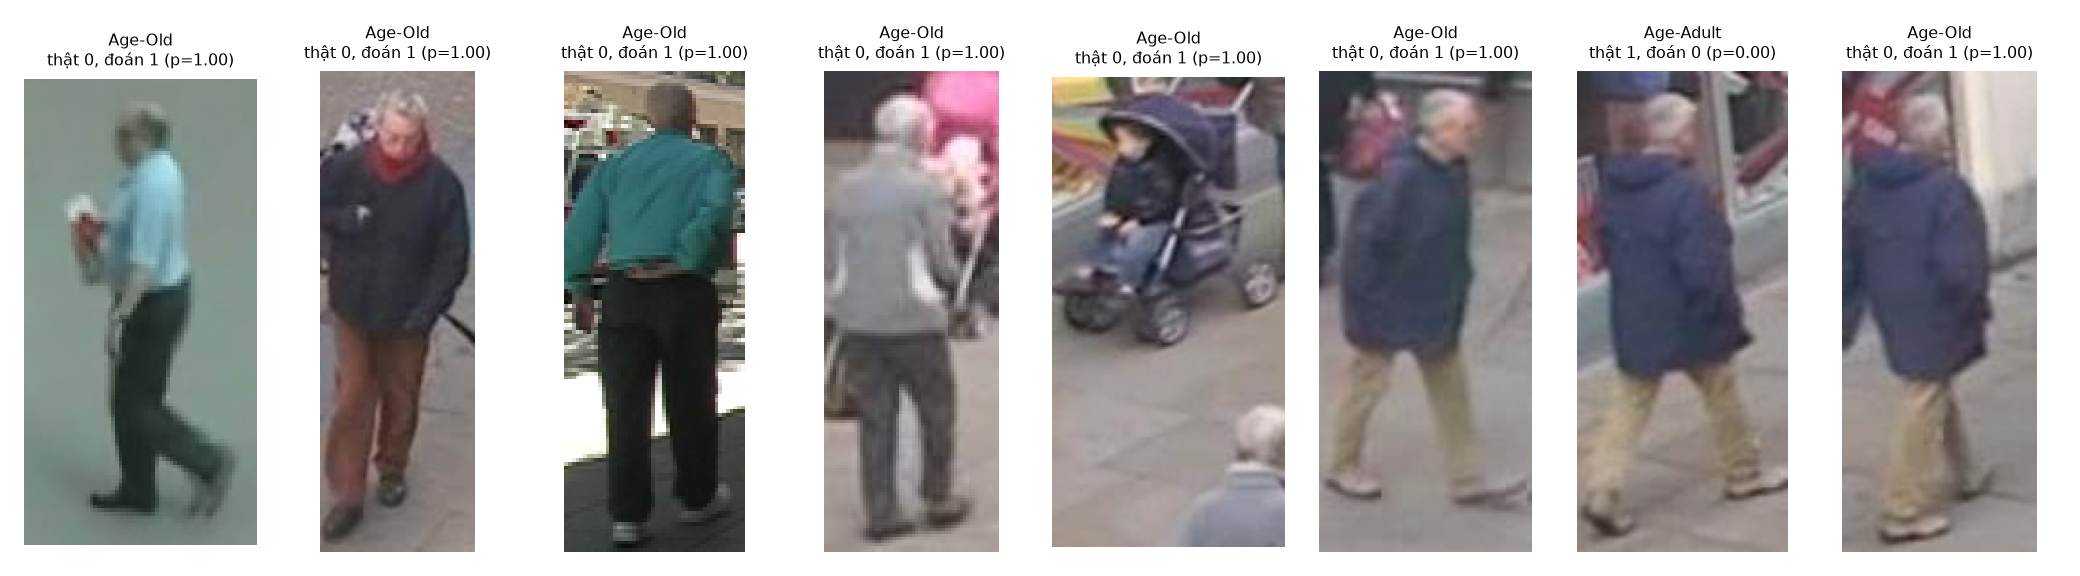
\includegraphics[width=\linewidth]{errors_PETA.png}
\caption{Các lỗi có độ tin cậy cao nhất ở nhóm tuổi trên PETA giấu. Mô hình trả lời với xác suất gần 0 hoặc gần 1 ngược với label. Nhiều ca trông giống lỗi label hoặc khác quy ước gán nhãn hơn là lỗi nhận dạng.}
\label{fig:errors}
\end{figure}

\paragraph{Cơ chế.} \textbf{Label smoothing} (tạm dịch: làm mềm nhãn) với hệ số $\epsilon=0.05$ đặt mục tiêu huấn luyện là 0.975 thay cho 1 và 0.025 thay cho 0. Binary cross-entropy (tạm dịch: entropy chéo nhị phân) đạt cực tiểu khi xác suất bằng mục tiêu, nên mô hình được khuyến khích ở trong khoảng $[0.025, 0.975]$. Mức phạt lớn nhất của một thuộc tính vì vậy vào khoảng $\log 0.025\approx-3.7$ thay cho $-9.2$ ở sàn $10^{-4}$. Trên 48 lần huấn luyện, nhiều nhất 0,52\% số ô trên camera giấu có xác suất dưới 0.025 cho giá trị đúng.

\paragraph{Kiểm tra độ nhạy.} Chúng tôi đảo ngược phép làm mềm trên logit đã huấn luyện, để mô hình trả về xác suất như thể không có label smoothing. mADM giảm 0.027, từ 0.6261 xuống 0.5990, dù mAP tăng nhẹ. Phép thử này không thay thế được một lần huấn luyện không làm mềm, vì mô hình đó sẽ học logit khác, và chúng tôi chưa chạy lần huấn luyện đó. Nó chỉ cho thấy điểm xếp hạng phụ thuộc mạnh vào sàn xác suất mà label smoothing tạo ra.

\subsection{Group CE cho các thuộc tính loại trừ nhau}
\label{sec:gce}

\paragraph{Vấn đề.} Phần lớn thuộc tính nằm trong năm nhóm mà mỗi người có đúng một giá trị, gồm ba nhóm tuổi, ba độ dài tóc, hai kiểu quần, 12 màu áo và 12 màu quần. Mô hình với 40 sigmoid độc lập không biết điều này. Trên PETA giấu, với những người có đúng một màu áo theo label, tổng 12 xác suất màu áo mà mô hình ViT-B trả về có trung bình 1.46 thay vì 1. Mô hình phân bố xác suất lên cả những cấu hình không thể xảy ra, như hai màu áo cùng lúc.

\paragraph{Cơ chế.} Với mỗi nhóm $\mathcal{G}$ mà ảnh $i$ có đúng một label dương $c$, chúng tôi thêm vào loss một số hạng \textbf{group cross-entropy} (group CE, tạm dịch: entropy chéo theo nhóm):
\begin{equation}
\mathcal{L}_{\text{GCE}}=-\frac{1}{n}\sum_{(i,\mathcal{G})}\log\frac{\exp z_{ic}}{\sum_{k\in\mathcal{G}}\exp z_{ik}},\qquad \mathcal{L}=\mathcal{L}_{\text{BCE}}+0.5\,\mathcal{L}_{\text{GCE}}.
\end{equation}
Phân số là softmax của các logit trong nhóm, lấy tại giá trị đúng. Số hạng này buộc logit của giá trị đúng tách khỏi logit của các giá trị khác cùng nhóm. Lúc inference (tạm dịch: suy luận), mô hình vẫn trả về 40 sigmoid độc lập và hàm xếp hạng không đổi. Hình~\ref{fig:gce} minh hoạ phép tính trên hai người PETA chọn ngẫu nhiên.

\begin{figure}[H]
\centering
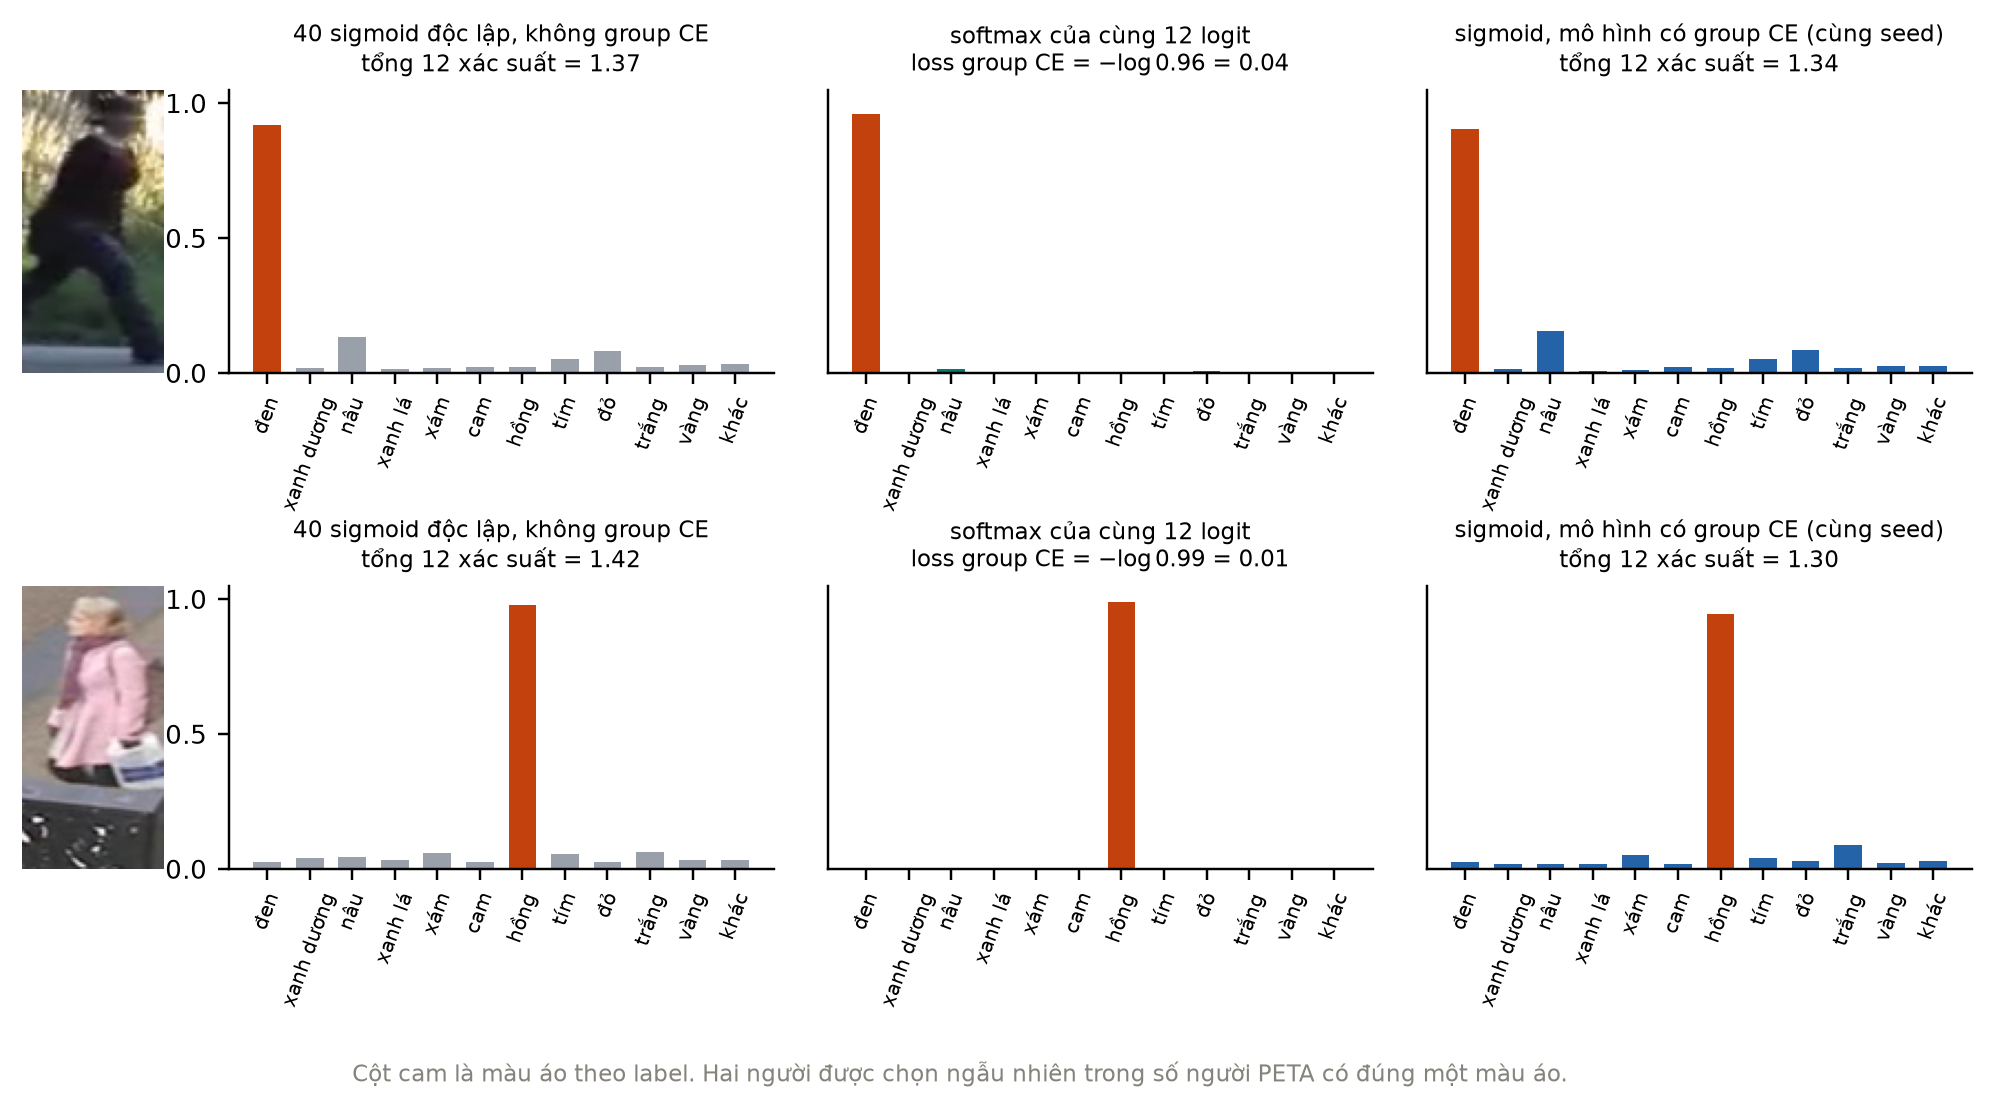
\includegraphics[width=\linewidth]{t2_gce_people.png}
\caption{Group CE trên 12 màu áo của hai người PETA chọn ngẫu nhiên. Cột trái là 12 xác suất sigmoid của mô hình không có group CE, có tổng lớn hơn 1. Cột giữa là softmax của cùng 12 logit, và loss group CE là $-\log$ của cột màu đúng. Cột phải là mô hình có group CE, cùng seed. Với hai người đã rõ màu như ở đây, loss gần 0 và xác suất gần như không đổi. Tác động trung bình của group CE nhỏ ở từng người và chỉ thấy được qua thống kê trên cả gallery (Bảng~\ref{tab:gce}).}
\label{fig:gce}
\end{figure}

\paragraph{Kết quả.} Bảng~\ref{tab:gce} liệt kê mọi cặp lần huấn luyện chỉ khác nhau ở số hạng này. mADM tăng ở cả 8 cặp, từ 0.0040 đến 0.0125, trong khi AUC tăng ở cặp này và giảm ở cặp khác. Phân rã NLL cho thấy hai cơ chế khác nhau. Trên PETA, gần như toàn bộ mức giảm NLL nằm ở phần calibration. Ở 6 cặp PETA, phần calibration trên camera giấu giảm 0.15 đến 0.23 nats, trong khi trên val của camera nguồn gần như không đổi. Group CE vì vậy giảm đúng phần sai lệch riêng của camera mới, điều mà phép sửa sau huấn luyện ở mục~\ref{sec:calib} không làm được. Trên Market1501, mức giảm lại nằm ở refinement. Chúng tôi chưa có giải thích được kiểm chứng cho hiệu ứng trên PETA. Một giả thuyết là softmax buộc các logit trong nhóm cạnh tranh nhau, nên một dịch chuyển chung của camera, ví dụ ánh màu làm mọi logit màu xám tăng, không đẩy được một màu lên tự do.

\begin{table}[H]
\centering\small
\resizebox{\linewidth}{!}{%
\begin{tabular}{@{}llcccccc@{}}
\toprule
Bộ giấu & Mô hình gốc & $\Delta$mADM & $\Delta$NLL & $\Delta$calibration & $\Delta$refinement & $\Delta$mADM sau oracle & $\Delta$AUC \\
\midrule
PETA & ViT-B query head (seed 2) & +0.0120 & $-$0.27 & $-$0.21 & $-$0.06 & +0.0028 & $-$0.0026 \\
PETA & ViT-B query head, noise adaptation & +0.0080 & $-$0.22 & $-$0.18 & $-$0.04 & +0.0022 & +0.0005 \\
PETA & ViT-B query head, che label nhiễu & +0.0040 & $-$0.17 & $-$0.15 & $-$0.02 & +0.0019 & +0.0030 \\
PETA & ViT-L query head, 5 epoch & +0.0125 & $-$0.21 & $-$0.18 & $-$0.02 & +0.0042 & +0.0032 \\
PETA & ViT-L linear head, 5 epoch & +0.0067 & $-$0.17 & $-$0.18 & +0.02 & +0.0015 & $-$0.0012 \\
PETA & ViT-L query head, 3 epoch & +0.0084 & $-$0.24 & $-$0.23 & $-$0.01 & +0.0014 & +0.0039 \\
Market & ViT-B query head & +0.0056 & $-$0.14 & $-$0.03 & $-$0.11 & +0.0036 & $-$0.0015 \\
Market & ViT-B query head, noise adaptation & +0.0062 & $-$0.11 & $-$0.01 & $-$0.10 & +0.0023 & +0.0032 \\
\bottomrule
\end{tabular}}
\caption{Group CE trên 8 cặp lần huấn luyện chỉ khác nhau ở số hạng này. NLL và hai phần của nó tính bằng nats. Trên PETA, mức giảm NLL gần như nằm hết ở phần calibration. Trên Market1501, nó nằm ở refinement.}
\label{tab:gce}
\end{table}

\subsection{Distillation từ hai teacher}
\label{sec:kd}

\paragraph{Vấn đề.} Giới hạn thời gian của máy chấm chỉ cho phép ViT-B chạy an toàn. Các mô hình lớn hơn cho xác suất tốt hơn rõ rệt. ViT-L 256×128 với linear head (tạm dịch: head tuyến tính) đạt NLL 6.57 và mADM 0.6697 trên PETA giấu, so với 6.98 và 0.6261 của ViT-B với query head, nhưng chạy chậm hơn khoảng 3,5 lần.

\paragraph{Cơ chế.} \textbf{Knowledge distillation} (tạm dịch: chưng cất kiến thức) huấn luyện mô hình nhỏ khớp với xác suất mềm của mô hình lớn~\cite{hinton}. Mô hình lớn gọi là \textbf{teacher} (tạm dịch: mô hình thầy), mô hình nộp bài gọi là \textbf{student} (tạm dịch: mô hình trò). Hai teacher là DINOv3-L ở 176×96 và CLIP-L/14~\cite{clip} ở 168×84, mỗi teacher được fine-tune (tạm dịch: tinh chỉnh) 3 epoch. Báo cáo Track 1 giải thích vì sao chọn hai mô hình khác họ pretrain. Loss của student là $(1-\alpha)\mathcal{L}_{\text{label}}+\alpha\,\mathcal{L}_{\text{KD}}$ với $\alpha=0.8$, trong đó $\mathcal{L}_{\text{KD}}$ là binary cross-entropy giữa xác suất của student và sigmoid của trung bình logit hai teacher. Theo Beyer và cộng sự~\cite{patient}, với xác suất 0.5, một batch được thay bằng ảnh trộn từ hai ảnh bằng mixup hoặc CutMix, và batch đó chỉ học từ teacher vì label thật không mô tả được ảnh trộn. Student học 20 epoch, lâu hơn khoảng hai lần so với khi không distillation.

\begin{figure}[H]
\centering
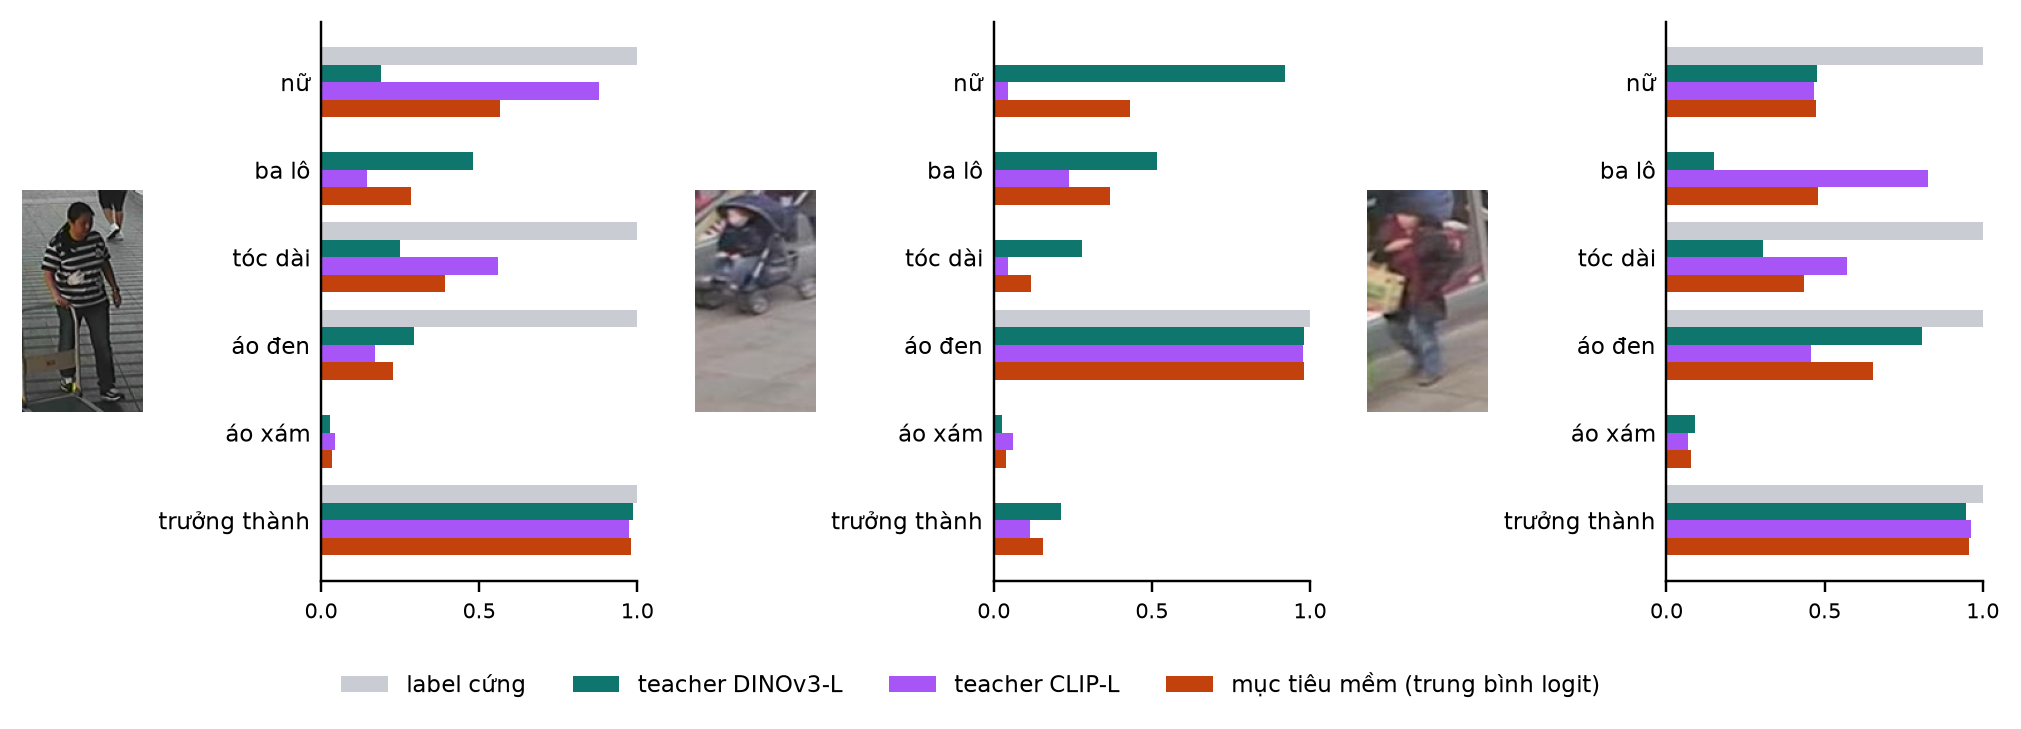
\includegraphics[width=\linewidth]{distill_targets.png}
\caption{Mục tiêu mà student học trên ba ảnh PETA. Thanh xám là label cứng, luôn là 0 hoặc 1. Thanh xanh lục và tím là xác suất của hai teacher được huấn luyện không có PETA. Thanh cam là mục tiêu mềm, sigmoid của trung bình hai logit. Ở những thuộc tính mà ảnh không rõ hoặc hai teacher bất đồng, mục tiêu mềm nằm giữa 0 và 1, nên student được dạy trả về xác suất vừa phải đúng ở những chỗ đó.}
\label{fig:distill}
\end{figure}

Hình~\ref{fig:distill} cho thấy vì sao distillation hợp với Track 2. Label cứng buộc student trả về 0 hoặc 1 kể cả khi ảnh không đủ rõ, và đó chính là nguồn của các lỗi tự tin ở Hình~\ref{fig:errors}. Mục tiêu mềm của teacher giữ xác suất ở mức vừa phải ở những ảnh khó, nên giảm các ô bị phạt nặng trong phương trình~\eqref{eq:ll}.

\paragraph{Kết quả.} Bảng~\ref{tab:kd} tách tác động của teacher khỏi tác động của độ dài huấn luyện, trên student ViT-L. Ở cùng 3 epoch, distillation cải thiện refinement 0.06 nats và mADM 0.0040, khoảng một rưỡi sai số chuẩn. Huấn luyện lâu hơn mà không có teacher làm refinement kém đi, từ 5.51 lên 5.58 nats khi đi từ 3 lên 5 epoch. Có teacher, refinement tiếp tục tốt lên, tới 5.41 nats ở 10 epoch, và mADM sau oracle tăng 0.012. Distillation vì vậy tác động lên refinement và làm cho huấn luyện dài trở nên có ích. Với ViT-B dùng khi nộp, distillation hai teacher với ảnh trộn trong 10 epoch nâng mADM trên PETA từ 0.6406 lên 0.6577, gần một ViT-L không distillation có group CE (0.6622). So sánh này lẫn cả độ dài huấn luyện, nên chúng tôi chỉ đọc nó là distillation thu hẹp phần lớn khoảng cách từ ViT-B lên ViT-L.

\begin{table}[H]
\centering\small
\begin{tabular}{@{}lcccccc@{}}
\toprule
Student ViT-L 176×96 & epoch & mADM & NLL & calibration & refinement & mADM sau oracle \\
\midrule
chỉ học label (2 lần chạy) & 3 & 0.6515 & 6.91 & 1.40 & 5.51 & 0.6783 \\
chỉ học label & 5 & 0.6496 & 6.77 & 1.19 & 5.58 & 0.6740 \\
DINOv3-L + CLIP-L & 3 & 0.6555 & 6.93 & 1.47 & 5.46 & 0.6789 \\
DINOv3-L + CLIP-L & 6 & 0.6635 & 6.69 & 1.26 & 5.43 & 0.6846 \\
DINOv3-L + CLIP-L & 10 & 0.6681 & 6.63 & 1.22 & 5.41 & 0.6906 \\
DINOv3-L + MetaCLIP2-H & 10 & 0.6697 & 6.61 & 1.22 & 5.40 & 0.6887 \\
\bottomrule
\end{tabular}
\caption{Distillation và độ dài huấn luyện trên PETA giấu, không có group CE. NLL và hai phần của nó tính bằng nats. Không có teacher, học lâu hơn làm refinement kém đi. Có teacher, refinement tiếp tục tốt lên tới 10 epoch.}
\label{tab:kd}
\end{table}

\subsection{Những thay đổi chỉ dời logit thì có hại}

Track 1 cộng một offset vào logit để đặt threshold hiệu dụng. Ở Track 2 không có threshold, và offset chỉ làm sai độ lớn của xác suất. Áp offset của Track 1 làm mADM giảm trên val cùng domain, nên gói nộp Track 2 dùng logit nguyên bản. Logit adjustment~\cite{logitadj} là ví dụ cực đoan hơn. Phương pháp này dời logit theo tần suất label để tối ưu balanced accuracy (tạm dịch: độ chính xác cân bằng). AUC của nó bình thường (0.9019), nhưng NLL tăng từ khoảng 7 lên 31,86 và mADM giảm 0.087 (Phụ lục~\ref{app:var}). Mọi thay đổi chủ yếu dời độ lớn của logit, dù có ích ở Track 1, đều có hại ở Track 2.

\begin{ghichu}
Ba thay đổi ở bước huấn luyện cải thiện ổn định trên mọi camera giấu đã đo. Label smoothing chặn mức phạt của một thuộc tính sai, group CE giảm phần sai lệch calibration riêng của camera mới trên PETA, và distillation cải thiện refinement khi huấn luyện dài. Không thay đổi nào trong ba thay đổi này cần biết hệ số chặn của camera chấm.
\end{ghichu}

%=====================================================================
\section{Lỗi còn lại nằm ở đâu}
\label{sec:errors}

\subsection{Ảnh nào đứng trước ảnh khớp chính xác}

Với mô hình ViT-L distillation trên PETA giấu, chúng tôi lấy các ảnh không khớp được xếp trước ảnh khớp chính xác đầu tiên của mỗi query, tối đa 10 ảnh cho một query, tổng cộng 8897 ảnh. Hình~\ref{fig:conf} cho biết các ảnh này lệch query ở thuộc tính nào và lệch bao nhiêu thuộc tính.

\begin{figure}[H]
\centering
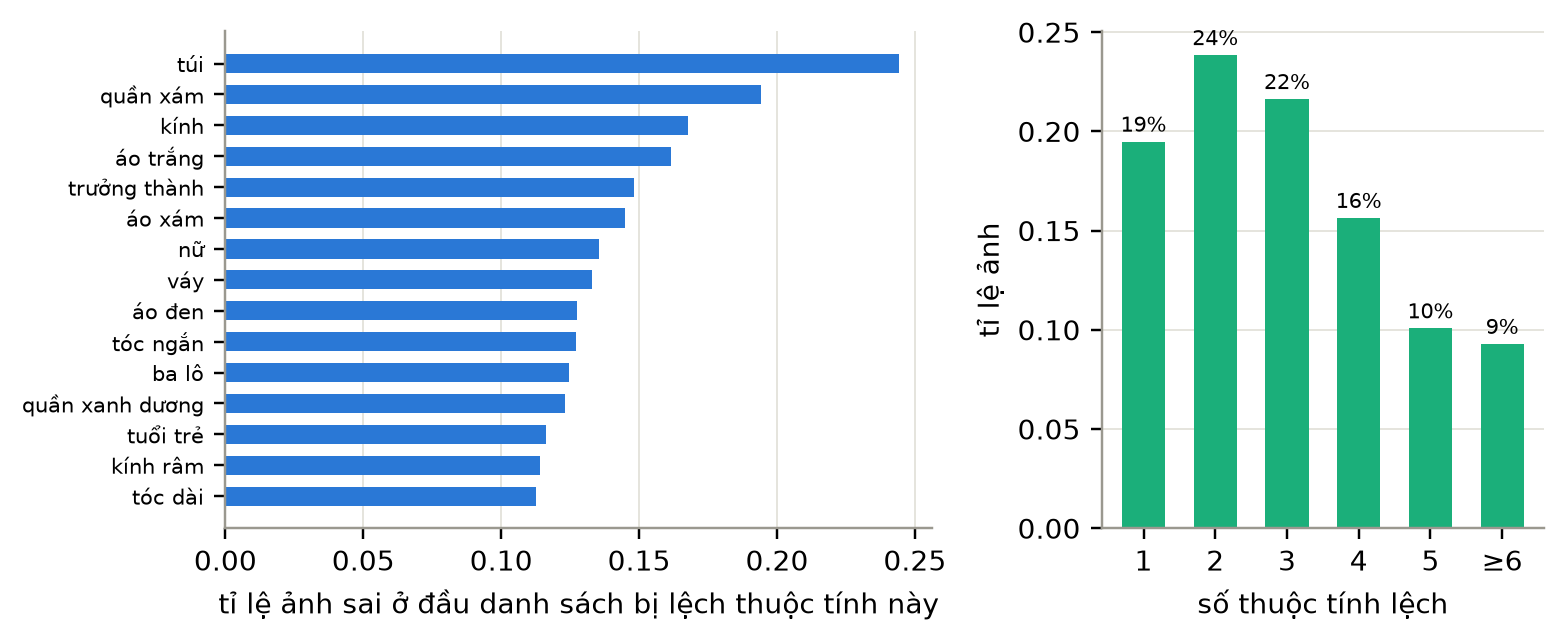
\includegraphics[width=\linewidth]{confusers.png}
\caption{Trái, 15 thuộc tính thường bị lệch nhất ở các ảnh không khớp nhưng đứng trước ảnh khớp đầu tiên. Phải, phân bố số thuộc tính lệch của các ảnh này. Gần một nửa chỉ lệch 1 hoặc 2 thuộc tính và vẫn nhận 0.72 đến 0.86 điểm ndom.}
\label{fig:conf}
\end{figure}

Ba nhóm nguyên nhân nổi lên. Nhóm thứ nhất là phụ kiện nhỏ, gồm túi (24\% số ảnh), kính (17\%), kính râm và ba lô. Ở 256×128, những vật này chỉ chiếm vài patch. Nhóm thứ hai là các màu trung tính, gồm quần xám (19\%), áo trắng (16\%), áo xám và áo đen. Ranh giới giữa xám, trắng và đen phụ thuộc vào ánh sáng và vào quy ước gán nhãn, và đây cũng là nhóm có lỗi threshold lớn nhất ở Track 1. Nhóm thứ ba là các thuộc tính có ranh giới chủ quan, gồm tuổi và độ dài tóc. Trung bình mỗi ảnh lệch 3.07 thuộc tính, và 43\% số ảnh chỉ lệch 1 hoặc 2 thuộc tính.

\subsection{Nhóm thuộc tính nào làm mất nhiều likelihood nhất}

NLL trên một ảnh là tổng của 40 thành phần, nên có thể tách theo nhóm thuộc tính (Hình~\ref{fig:nllg}).

\begin{figure}[H]
\centering
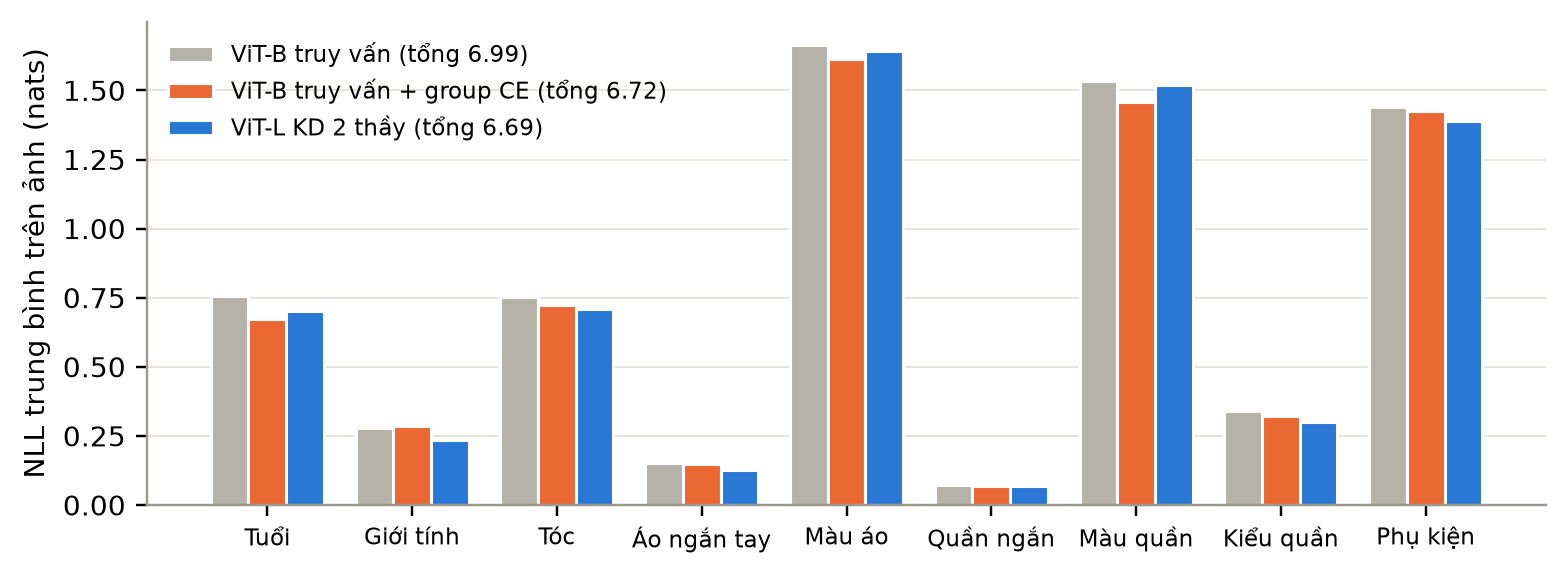
\includegraphics[width=\linewidth]{nll_groups.png}
\caption{NLL trung bình trên một ảnh, tách theo nhóm thuộc tính, trên PETA giấu. Ba mô hình là cặp ViT-B cùng seed không có và có group CE, cùng một ViT-L distillation. Màu áo, màu quần và phụ kiện chiếm khoảng hai phần ba tổng NLL.}
\label{fig:nllg}
\end{figure}

Hai nhóm màu và nhóm phụ kiện chiếm khoảng 4,6 trên 7,0 nats của mô hình ViT-B, nên mọi cải thiện có ý nghĩa phải đi qua ba nhóm này. Ở cặp cùng seed, group CE giảm tổng NLL 0.27 nats, và khoảng 90\% mức giảm nằm ở tuổi, tóc và hai nhóm màu, đúng các nhóm mà số hạng này tác động. Mô hình ViT-L distillation giảm NLL ở giới tính, áo ngắn tay, kiểu quần và phụ kiện nhiều hơn ở các nhóm màu. So sánh này gộp hai thay đổi là backbone lớn hơn và distillation, nên chỉ gợi ý rằng group CE và distillation bổ sung cho nhau.

\subsection{Độ khó của từng query}

\begin{figure}[H]
\centering
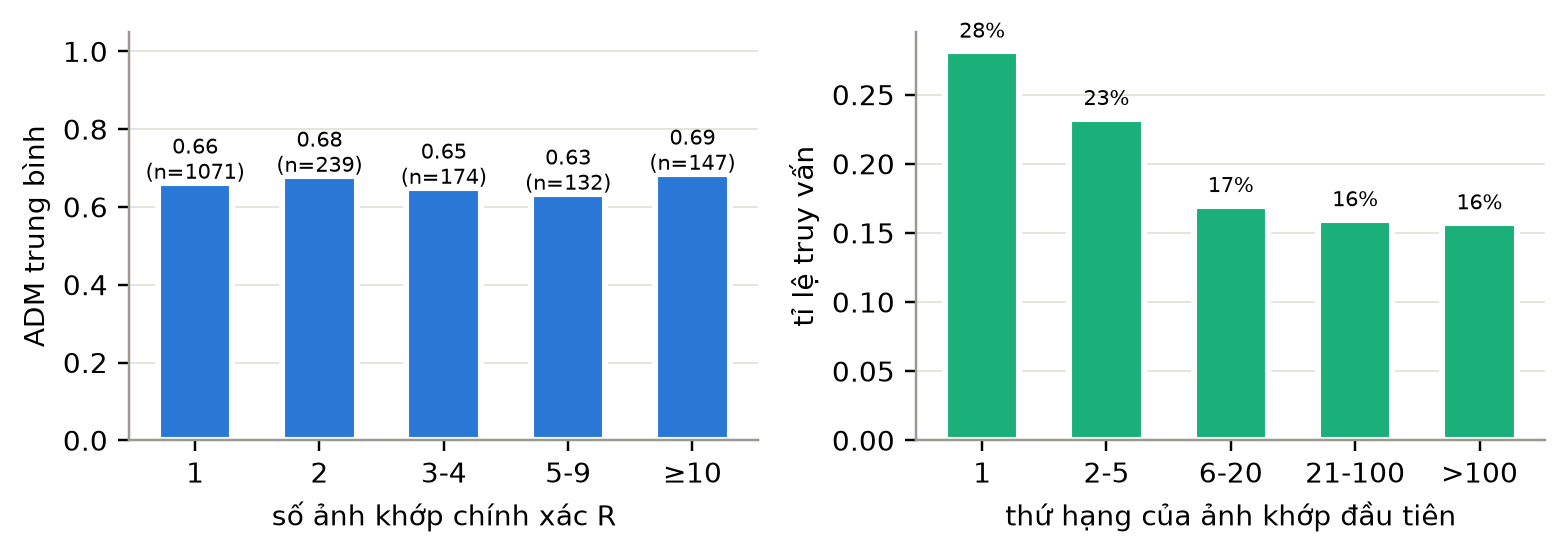
\includegraphics[width=\linewidth]{query_difficulty.png}
\caption{Trái, ADM trung bình theo số ảnh khớp chính xác của query. Phải, phân bố thứ hạng của ảnh khớp đầu tiên. ADM gần như không đổi theo số ảnh khớp, và 16\% query có ảnh khớp đầu tiên nằm sau hạng 100.}
\label{fig:diff}
\end{figure}

Hình~\ref{fig:diff} phân tích 1763 query của PETA giấu. ADM gần như không phụ thuộc vào số ảnh khớp (0.63 đến 0.69 ở mọi nhóm). Nó phụ thuộc mạnh vào vị trí của ảnh khớp đầu tiên, với trung bình 0.90 khi ảnh này đứng hạng 1 và 0.40 khi nó nằm sau hạng 100. Ở những query khó nhất, AP gần bằng 0 và phần điểm còn lại gần như toàn bộ đến từ các ảnh khớp gần.

%=====================================================================
\section{Kết quả trên hidden test set}
\label{sec:lb}

\begin{figure}[H]
\centering
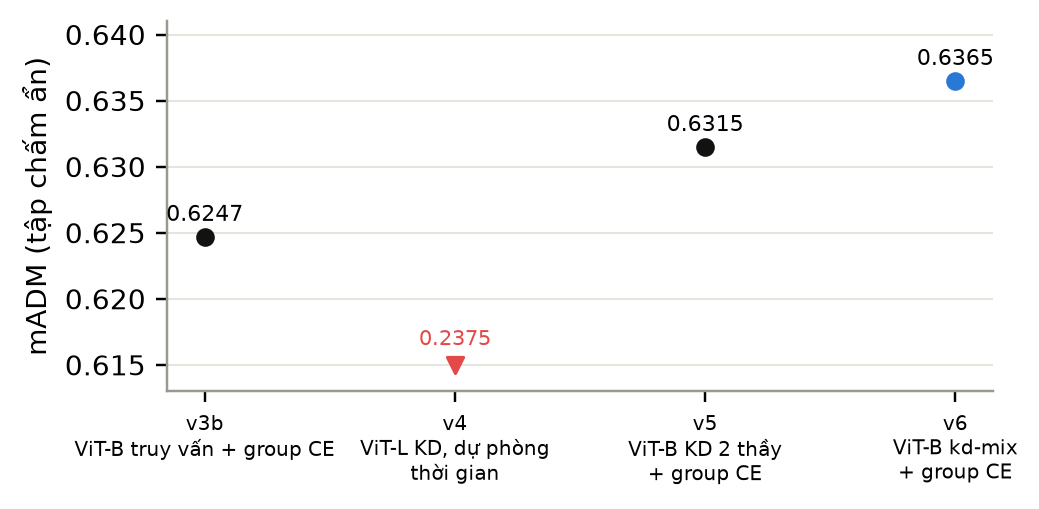
\includegraphics[width=0.62\linewidth]{leaderboard.png}
\caption{mADM trên hidden test set của các bài nộp có ghi nhận kết quả. Bài v4 bị cơ chế dự phòng thời gian làm hỏng. Hai bước distillation (v5 và v6) mỗi bước tăng khoảng 0.005 đến 0.007.}
\label{fig:lb}
\end{figure}

\begin{table}[H]
\centering\small
\begin{tabularx}{\linewidth}{@{}llXc@{}}
\toprule
Bài & Mô hình & Thành phần chính & Test set \\
\midrule
v1 & ViT-L 176, query head & mô hình Track 1, $s_{LL}$ & không ghi nhận \\
v2 & ViT-B, query head & train và val & không ghi nhận \\
v3b & ViT-B, query head & thêm group CE, train và val & 0.6247 \\
v4 & ViT-L 176, query head & distillation hai teacher, có dự phòng thời gian & 0.2375 \\
v5 & ViT-B, query head & group CE và distillation hai teacher, 10 epoch & 0.6315 \\
v6 & ViT-B, query head & group CE và distillation có ảnh trộn, 20 epoch, không dự phòng & 0.6365 \\
\bottomrule
\end{tabularx}
\caption{Các bài nộp Track 2. Từ v3b sang v5 và từ v5 sang v6, mỗi bước đổi hai yếu tố.}
\label{tab:lb}
\end{table}

\paragraph{Mức tăng trên test set.} Từ v3b sang v5, thêm distillation hai teacher và lịch 10 epoch, mADM tăng 0.0068. Từ v5 sang v6, thêm ảnh trộn và lịch 20 epoch, mADM tăng thêm 0.0050. Mỗi bước đổi hai yếu tố, nên chúng tôi không quy mức tăng cho một nguyên nhân duy nhất. Cả hai bước đều dương, lớn hơn noise (tạm dịch: nhiễu) giữa các lần huấn luyện lặp, và cùng chiều với Bảng~\ref{tab:kd}. Điểm baseline 2027 của ban tổ chức không được công khai.

\paragraph{Thất bại do cơ chế dự phòng.} Bài v4 dùng ViT-L 176 distillation. Trên một lần chạy máy chấm chậm, ViT-L mất 176 đến 190 ms một ảnh thay vì khoảng 103 ms như lần trước, và chương trình vượt ngân sách thời gian nội bộ. Cơ chế dự phòng khi đó gán xác suất trung bình của tập train cho mọi ảnh còn lại. Các ảnh này nhận cùng một điểm với mọi query, tạo thành một khối lớn điểm bằng nhau, và mADM rơi xuống 0.2375. Bản cuối bỏ hẳn cơ chế dự phòng. Một bài thất bại giữ nguyên điểm cũ trên leaderboard (tạm dịch: bảng xếp hạng), còn một bài dự phòng thay điểm tốt bằng điểm xấu. Mọi bài nộp sau đó dùng ViT-B, vốn chạy kịp ở cả những lần máy chậm nhất đã quan sát.

%=====================================================================
\section{Bài học}
\label{sec:lessons}

\paragraph{Câu trả lời cho câu hỏi ở tiêu đề.} Một nửa. Sai lệch calibration làm mất 0.018 đến 0.057 mADM trên camera giấu, nhiều hơn mọi thay đổi huấn luyện chúng tôi tìm được, nên chẩn đoán của ban tổ chức chỉ ra một tổn thất có thật. Nhưng phần lớn tổn thất này có sẵn từ cách huấn luyện, và phần mà camera mới thêm vào là hệ số chặn của từng thuộc tính, thứ dữ liệu nguồn không ước lượng được.

\paragraph{Cùng một kỹ thuật, hai kết quả trái ngược.} Track 1 và Track 2 dùng chung dữ liệu, chung mô hình và chung ràng buộc tính toán, nên là một cặp đối chứng tự nhiên. Bảng~\ref{tab:t1t2} đặt cạnh nhau tác động của cùng một kỹ thuật lên hai track. Offset khớp trên camera nguồn có ích ở Track 1 và có hại ở Track 2. Các kỹ thuật cải thiện xác suất mà không dời threshold, gồm group CE, ensemble (tạm dịch: tổ hợp mô hình) và distillation, có ích ở Track 2 nhiều hơn hẳn ở Track 1.

\begin{table}[H]
\centering\small
\begin{tabularx}{\linewidth}{@{}Xcc@{}}
\toprule
Kỹ thuật (PETA giấu) & Track 1, thay đổi Avg & Track 2, thay đổi mADM \\
\midrule
Offset khớp trên camera nguồn × 0.6 & +0.007 & giảm trên val cùng domain \\
Logit adjustment & $-0.122$ & $-0.087$ \\
Group CE (8 cặp) & $-0.005$ đến +0.003 & +0.004 đến +0.0125 \\
Ensemble hai mô hình ViT-B & $-0.002$ đến +0.0004 & +0.005 đến +0.020 \\
Distillation hai teacher (student ViT-B) & +0.004 & +0.017 \\
\bottomrule
\end{tabularx}
\caption{Tác động của cùng một kỹ thuật lên hai track. Offset giúp Track 1 và hại Track 2. Các kỹ thuật cải thiện xác suất giúp Track 2 nhiều hơn hẳn Track 1.}
\label{tab:t1t2}
\end{table}

\paragraph{Bốn điều nên làm.}
\begin{enumerate}[leftmargin=1.6em]
\item Xếp hạng bằng log-likelihood của đúng vector query, không bằng khoảng cách L1.
\item Chọn mô hình bằng NLL hoặc mADM trên một domain giấu, không bằng AUC hay điểm sau threshold.
\item Không sửa calibration bằng tham số học trên camera nguồn. Hệ số chặn học được ở đó không đúng cho camera mới.
\item Đưa cải thiện vào bước huấn luyện, qua label smoothing, loss theo nhóm thuộc tính loại trừ và distillation với lịch dài.
\end{enumerate}

\paragraph{Vì sao các đội trước khó vượt baseline.} Kết quả của chúng tôi gợi ý thêm một giải thích cho nhận định của ban tổ chức~\cite{upar24}. Các mô hình nhận dạng thuộc tính mạnh thường được tối ưu cho chỉ số ở threshold cố định, bằng các kỹ thuật dời threshold như logit adjustment, weight mạnh cho thuộc tính hiếm hoặc khớp offset. Các kỹ thuật này giữ nguyên AUC nhưng làm hỏng độ lớn của xác suất, và với hàm xếp hạng L1 hay log-likelihood, độ lớn đó chính là thứ quyết định thứ hạng.

\paragraph{Ràng buộc của luật thi.}
\label{sec:rules}
Tập query của test set được tạo từ chính các vector label của gallery. Mọi thống kê tính chéo nhiều query, như thuộc tính nào luôn bằng 0, vì vậy là thống kê trên label của test set. Trên val, hai kỹ thuật dạng này tăng mADM 0.002 đến 0.005. Chúng tôi không dùng chúng vì chúng đi ngược tinh thần của luật cấm dùng thông tin của test set. Chấm từng query độc lập luôn hợp lệ.

\paragraph{Giới hạn.} Phần lớn số liệu dựa trên PETA giấu, và PA100k chỉ có hai lần huấn luyện. Label smoothing chưa được ablation ở bước huấn luyện. So sánh distillation cho ViT-B lẫn cả độ dài huấn luyện. Phương trình~\eqref{eq:ll} giả sử các thuộc tính độc lập khi biết ảnh, trong khi group CE cố ý vi phạm giả thiết này lúc huấn luyện.

\paragraph{Tác động xã hội.} Truy xuất người theo các thuộc tính như tuổi và giới tính trên video giám sát có thể bị dùng để theo dõi cá nhân mà không có sự đồng ý. Báo cáo chỉ trình bày kết quả kỹ thuật và không công bố mô hình đã huấn luyện.

\begin{thebibliography}{99}\small
\bibitem{upar} A.~Specker, M.~Cormier, J.~Beyerer. UPAR: Unified pedestrian attribute recognition and person retrieval. \textit{WACV}, 2023.
\bibitem{upar23} M.~Cormier, A.~Specker, J.~C.~S.~Jacques Junior và cộng sự. UPAR challenge: Pedestrian attribute recognition and attribute-based person retrieval, dataset, design, and results. \textit{WACV Workshops}, 2023.
\bibitem{upar24} M.~Cormier, A.~Specker, J.~C.~S.~Jacques Junior và cộng sự. UPAR challenge 2024: Pedestrian attribute recognition and attribute-based person retrieval, dataset, design, and results. \textit{WACV Workshops}, 2024.
\bibitem{specker21} A.~Specker, J.~Beyerer. Improving attribute-based person retrieval by using a calibrated, weighted, and distribution-based distance metric. \textit{ICIP}, 2021.
\bibitem{specker23} A.~Specker, J.~Beyerer. Balanced pedestrian attribute recognition for improved attribute-based person retrieval. \textit{ICPRS}, 2023.
\bibitem{pa100k} X.~Liu, H.~Zhao, M.~Tian và cộng sự. HydraPlus-Net: Attentive deep features for pedestrian analysis. \textit{ICCV}, 2017.
\bibitem{market} L.~Zheng, L.~Shen, L.~Tian và cộng sự. Scalable person re-identification: A benchmark. \textit{ICCV}, 2015.
\bibitem{peta} Y.~Deng, P.~Luo, C.~C.~Loy, X.~Tang. Pedestrian attribute recognition at far distance. \textit{ACM Multimedia}, 2014.
\bibitem{cuhkpedes} S.~Li, T.~Xiao, H.~Li và cộng sự. Person search with natural language description. \textit{CVPR}, 2017.
\bibitem{guo} C.~Guo, G.~Pleiss, Y.~Sun, K.~Q.~Weinberger. On calibration of modern neural networks. \textit{ICML}, 2017.
\bibitem{ovadia} Y.~Ovadia, E.~Fertig, J.~Ren và cộng sự. Can you trust your model's uncertainty? Evaluating predictive uncertainty under dataset shift. \textit{NeurIPS}, 2019.
\bibitem{gneiting} T.~Gneiting, A.~E.~Raftery. Strictly proper scoring rules, prediction, and estimation. \textit{Journal of the American Statistical Association}, 2007.
\bibitem{prp} S.~E.~Robertson. The probability ranking principle in IR. \textit{Journal of Documentation}, 1977.
\bibitem{degroot} M.~H.~DeGroot, S.~E.~Fienberg. The comparison and evaluation of forecasters. \textit{Journal of the Royal Statistical Society, Series D}, 1983.
\bibitem{kull} M.~Kull, P.~Flach. Novel decompositions of proper scoring rules for classification: Score adjustment as precursor to calibration. \textit{ECML-PKDD}, 2015.
\bibitem{dap} C.~H.~Lampert, H.~Nickisch, S.~Harmeling. Learning to detect unseen object classes by between-class attribute transfer. \textit{CVPR}, 2009.
\bibitem{kreciprocal} Z.~Zhong, L.~Zheng, D.~Cao, S.~Li. Re-ranking person re-identification with k-reciprocal encoding. \textit{CVPR}, 2017.
\bibitem{hinton} G.~Hinton, O.~Vinyals, J.~Dean. Distilling the knowledge in a neural network. \textit{arXiv:1503.02531}, 2015.
\bibitem{patient} L.~Beyer, X.~Zhai, A.~Royer và cộng sự. Knowledge distillation: A good teacher is patient and consistent. \textit{CVPR}, 2022.
\bibitem{dinov3} O.~Siméoni, H.~V.~Vo, M.~Seitzer và cộng sự. DINOv3. \textit{arXiv:2508.10104}, 2025.
\bibitem{clip} A.~Radford, J.~W.~Kim, C.~Hallacy và cộng sự. Learning transferable visual models from natural language supervision. \textit{ICML}, 2021.
\bibitem{logitadj} A.~K.~Menon, S.~Jayasumana, A.~S.~Rawat và cộng sự. Long-tail learning via logit adjustment. \textit{ICLR}, 2021.
\end{thebibliography}

\appendix
\section{Bảng thuật ngữ}
\label{app:glossary}

\begin{table}[H]
\centering\small
\begin{tabularx}{\linewidth}{@{}lX@{}}
\toprule
Thuật ngữ & Ý nghĩa trong báo cáo \\
\midrule
retrieval & truy xuất, sắp xếp một kho ảnh theo mức phù hợp với một mô tả \\
query & truy vấn, vector 40 số 0 hoặc 1 mô tả người cần tìm \\
gallery & kho ảnh cần tìm, mỗi ảnh là một người đã cắt sẵn \\
ranking & xếp hạng, thứ tự ảnh do hệ thống trả về \\
khớp chính xác & ảnh có label bằng query ở cả 40 thuộc tính \\
mAP, mADM & chỉ số xếp hạng. mADM cộng thêm điểm cho ảnh khớp gần \\
domain & miền dữ liệu, ở đây là ảnh của một hệ thống camera \\
leave-one-dataset-out & huấn luyện trên hai bộ dữ liệu và đo trên bộ thứ ba \\
logit & số thực mà mô hình trả về trước sigmoid \\
log-likelihood $s_{LL}$ & log xác suất ảnh có đúng vector query, tổng 40 số hạng log \\
calibration & mức khớp giữa xác suất mô hình nói và tần suất thật \\
reliability diagram & biểu đồ tần suất thật theo xác suất mô hình trả về \\
Platt scaling & sửa calibration bằng $\sigma(a_kz_k+b_k)$ cho từng thuộc tính \\
hệ số dốc $a_k$, hệ số chặn $b_k$ & hai tham số của Platt scaling. $a_k$ làm sắc hoặc mềm, $b_k$ dời lên hoặc xuống \\
temperature scaling & Platt scaling với một $a$ chung và $b=0$, viết $T=1/a$ \\
NLL & log-likelihood âm của vector label đầy đủ, trung bình trên ảnh, đơn vị nats \\
phần calibration, refinement & hai phần của NLL. Phần đầu là lượng Platt oracle loại được, phần sau là lượng còn lại \\
oracle & phép đo dùng label của chính camera chấm, không làm được trong thực tế \\
label smoothing & làm mềm label 0 và 1 thành 0.025 và 0.975 \\
group CE & entropy chéo trên softmax của một nhóm thuộc tính loại trừ nhau \\
distillation, teacher, student & huấn luyện mô hình nhỏ (student) khớp xác suất của mô hình lớn (teacher) \\
ensemble & lấy trung bình logit của nhiều mô hình \\
\bottomrule
\end{tabularx}
\caption{Thuật ngữ dùng trong báo cáo.}
\end{table}

\section{Cấu hình bài nộp}

\begin{table}[H]
\centering\small
\begin{tabularx}{\linewidth}{@{}lX@{}}
\toprule
Thành phần & Giá trị (bài nộp v6) \\
\midrule
Backbone & \texttt{vit\_base\_patch16\_dinov3.lvd1689m}, 256×128 \\
Head & query head, 1 layer \\
Loss label & BCE, label smoothing 0.05, weight DeepMAR, cộng 0.5 × group CE \\
Distillation & teacher DINOv3-L 176×96 và CLIP-L/14 168×84 (train và val), $\alpha=0.8$, $T=1$ \\
Ảnh trộn & xác suất 0.5 cho mỗi batch, mixup Beta(0.8, 0.8) hoặc CutMix Beta(1, 1), 20 epoch \\
Tối ưu & AdamW, learning rate $5\cdot10^{-5}$ ở block cuối với layer decay 0.75, head gấp 10, weight decay 0.05, batch 64, warmup 0,5 epoch, cosine, EMA 0.9995 \\
Dữ liệu & train và val của cả ba bộ \\
Inference & logit nguyên bản, không offset, không temperature, không dự phòng thời gian \\
\bottomrule
\end{tabularx}
\caption{Cấu hình của bài nộp Track 2 tốt nhất.}
\end{table}

\section{Thuật toán xếp hạng}
\label{app:algo}

Phương trình~\eqref{eq:ll} viết lại được thành
\begin{equation}
s_{LL}(q,g)=q^{\top}\Big(\log\frac{p_g}{1-p_g}\Big)+\sum_k\log(1-p_{gk}).
\end{equation}
Số hạng thứ nhất là tích vô hướng giữa query và vector log-odds của ảnh. Số hạng thứ hai chỉ phụ thuộc vào ảnh. Hàm \texttt{rank\_gallery} của gói nộp làm các bước sau.

\begin{enumerate}[leftmargin=1.6em]
\item Với mỗi batch ảnh gallery, đọc ảnh, đổi kích thước về 256×128, chuẩn hoá theo ImageNet, chạy mô hình và lấy 40 logit.
\item Tính xác suất và kẹp vào $[10^{-4},1-10^{-4}]$.
\item Tính hai ma trận $L^{+}=\log P$ và $L^{-}=\log(1-P)$, mỗi ma trận kích thước $G\times40$.
\item Tính $S=Q\,(L^{+}-L^{-})^{\top}+\mathbf{1}\,(L^{-}\mathbf{1})^{\top}$, kích thước $|Q|\times G$, bằng một phép nhân ma trận float64.
\item Chuyển sang float32 và trả về dưới khoá \texttt{distances} giá trị $-S$, vì chương trình chấm coi giá trị nhỏ hơn là khớp hơn. Khoá này được đối chiếu với chương trình mẫu của ban tổ chức, vì một khoá sai sẽ đảo ngược toàn bộ thứ hạng.
\end{enumerate}

Với khoảng 3500 query và 29 nghìn ảnh, ma trận float64 chiếm khoảng 0,8 GB và vẫn nằm trong giới hạn bộ nhớ của máy chấm.

\section{Các hàm xếp hạng khác đã thử}
\label{app:scores}

\begin{table}[H]
\centering\small
\begin{tabularx}{\linewidth}{@{}Xcc@{}}
\toprule
Hàm xếp hạng (ViT-B query head, PETA giấu) & mADM & mAP \\
\midrule
L1, baseline~\cite{upar} & 0.57 đến 0.58 & \\
log-likelihood $s_{LL}$ (dùng trong bài nộp) & 0.6261 & 0.2773 \\
$s_{LL}$ với temperature $T=1.25$ & 0.6309 & 0.2717 \\
$s_{LL}$ với temperature khớp trên val camera nguồn ($T\approx0.8$) & giảm 0.004 đến 0.009 & \\
$s_{LL}$ cộng $0.5\log\sum_j e_j\,\ndom_j$ (mức khớp gần kỳ vọng) & 0.6290 & 0.2743 \\
$s_{LL}$ chỉ với mức khớp gần kỳ vọng & giảm 0.045 & \\
$s_{LL}$ với sàn xác suất 0.05 cho mọi thuộc tính & 0.6251 & 0.2631 \\
$s_{LL}$ với softmax trong từng nhóm loại trừ & 0.6139 & 0.2744 \\
$s_{LL}$ sau khi đảo ngược label smoothing & 0.5990 & 0.2826 \\
\bottomrule
\end{tabularx}
\caption{Các hàm xếp hạng trên PETA giấu. Các biến thể của log-likelihood dao động trong khoảng $\pm0.005$, trừ việc đảo ngược label smoothing, vốn làm mADM giảm 0.027.}
\label{tab:scores}
\end{table}

Số hạng mức khớp gần kỳ vọng được tính chính xác theo phân phối Poisson nhị thức. Gọi $m_k=q_k(1-p_k)+(1-q_k)p_k$ là xác suất thuộc tính $k$ lệch, và $r_k=m_k/(1-m_k)$. Xác suất lệch đúng $j$ thuộc tính là $e^{s_{LL}}\,e_j(r)$, với $e_j$ là đa thức đối xứng sơ cấp bậc $j$, tính từ các tổng luỹ thừa $\sum_k r_k^t$ bằng đẳng thức Newton. Số hạng này tăng mADM 0.003, nằm trong noise. Ép ràng buộc nhóm ở bước chấm điểm bằng softmax làm mADM giảm 0.005 đến 0.012 trên 5 mô hình, trong khi cùng ràng buộc đưa vào lúc huấn luyện (mục~\ref{sec:gce}) làm mADM tăng.

\section{Biến thể mô hình và ensemble}
\label{app:var}

\begin{table}[H]
\centering\small
\begin{tabular}{@{}lccc@{}}
\toprule
Biến thể (PETA giấu) & AUC & NLL / ảnh & mADM \\
\midrule
ViT-L 256×128, linear head & 0.9126 & 6.569 & 0.6697 \\
ViT-B query head + group CE & 0.9048 & 6.771 & 0.6424 \\
ViT-B query head, 3 epoch & 0.9041 & 7.102 & 0.6350 \\
ViT-L 160×80, linear head & 0.8960 & 6.823 & 0.6335 \\
ViT-B linear head, distillation logit từ ViT-L & 0.9028 & 6.861 & 0.6334 \\
ViT-B linear head & 0.9076 & 6.993 & 0.6313 \\
ViT-B query head + cân bằng trắng & 0.9001 & 6.985 & 0.6294 \\
PE-Core, linear head & 0.8950 & 6.916 & 0.6276 \\
ViT-B query head 2 layer & 0.9020 & 7.013 & 0.6270 \\
ViT-B query head, lần 1 và lần 2 & 0.9007 và 0.9040 & 6.976 và 6.998 & 0.6261 và 0.6254 \\
ViT-B head kép & 0.9041 & 7.037 & 0.6260 \\
ViT-B query head, đọc token 4 layer & 0.8988 & 6.997 & 0.6242 \\
ViT-B query head, cân bằng bộ dữ liệu & 0.9049 & 7.008 & 0.6214 \\
ViT-B logit adjustment & 0.9019 & 31.86 & 0.5396 \\
\bottomrule
\end{tabular}
\caption{Biến thể mô hình trên PETA giấu, xếp theo mADM (đợt chạy cũ). Logit adjustment có AUC bình thường nhưng NLL tăng gấp 4,5 lần và mADM giảm mạnh.}
\label{tab:var}
\end{table}

Trong đợt chạy này, linear head có AUC và mADM cao hơn query head ở ViT-B, nhưng các cặp cùng seed về sau cho kết quả đổi dấu giữa các camera giấu, nên chúng tôi không kết luận gì về head. Query head được giữ vì nó là nền của group CE và distillation.

\begin{table}[H]
\centering\small
\begin{tabular}{@{}lccc@{}}
\toprule
Ensemble logit (PETA giấu) & AUC & mADM & Avg Track 1 \\
\midrule
ViT-B query head & 0.9007 & 0.6261 & 0.7961 \\
ViT-B query head, hai lần huấn luyện & 0.9044 & 0.6315 & 0.7965 \\
ViT-B query head + ViT-B linear head & 0.9099 & 0.6389 & 0.7956 \\
ViT-B group CE + ViT-B linear head & 0.9108 & 0.6465 & 0.7945 \\
ViT-L 160 linear head + ViT-B group CE & 0.9090 & 0.6601 & \\
ViT-L 256 linear head + ViT-B group CE & 0.9173 & 0.6783 & 0.8028 \\
\bottomrule
\end{tabular}
\caption{Ensemble logit của các mô hình cùng họ DINOv3 trên PETA giấu. Ensemble tăng mADM 0.005 đến 0.052 trong khi Avg của Track 1 gần như không đổi. Ensemble tốn thời gian CPU của mọi mô hình thành phần, nên bài nộp dùng distillation để đưa một phần lợi ích này vào một ViT-B.}
\label{tab:ensb}
\end{table}

\section{Mã nguồn}

Mã nằm trong thư mục \texttt{track2/} của kho \texttt{upar-challenge-2027}. Hàm xếp hạng và chỉ số nằm ở \texttt{par/upar/retrieval.py}, đánh giá theo từng gallery ở \texttt{par/eval\_retrieval.py}, và group CE ở \texttt{par/upar/losses.py}. Các hình của báo cáo được tạo bởi \texttt{report/paper/make\_figs.py} và \texttt{report/paper/make\_process\_figs.py}.

\end{document}
